
%%%%%%%%%%%%%%%%%%%%%%% file main.tex %%%%%%%%%%%%%%%%%%%%%%%%
%
% Article à déposer pour TACAS 2015
%
%%%%%%%%%%%%%%%%%%%%%%%%%%%%%%%%%%%%%%%%%%%%%%%%%%%%%%


\documentclass[runningheads,a4paper]{llncs}

\usepackage{amssymb}
\setcounter{tocdepth}{3}
\usepackage{graphicx}

\usepackage{url}

%%%%%%%%%%%%%%%%%% Packages %%%%%%%%%%%%%%%%%%%%%%%%%
\usepackage{hyperref}


\usepackage{amsmath}  % Maths
\usepackage{amsfonts} % Maths
\usepackage{amssymb}  % Maths
\usepackage{stmaryrd} % Maths (crochets doubles)
\usepackage{ dsfont }

\usepackage{algorithm}
\usepackage{algpseudocode}


%%%%%%%%%%%%%%%%%%%%
\usepackage{listings}
% Définition du langage ASP
\lstdefinelanguage{ASP}{\^^M}
}

% Définition des styles de tous les listings du document
\lstset{language=ASP,
basicstyle=\small,
columns=flexible,
keywordstyle=\bfseries,
firstnumber=last
}
\renewcommand{\thelstnumber}{\the\value{lstnumber}}
%% fin définition

%%%%%%%%%%%%%%%%%%%%%%%%%%%%%%%%%%
\usepackage{enumerate} % Personnalisation de la numérotation des listes
\usepackage{url}     % Mise en forme + liens pour URLs
\usepackage{array}   % Tableaux évolués
\usepackage{comment}
\usepackage{moresize}
\usepackage{setspace}

\usepackage{prettyref}
\newrefformat{def}{Definition~\ref{#1}}
\newrefformat{fig}{Figure~\ref{#1}}
\newrefformat{pro}{Property~\ref{#1}}
\newrefformat{pps}{Proposition~\ref{#1}}
\newrefformat{lem}{Lemma~\ref{#1}}
\newrefformat{th}{Theorem~\ref{#1}}
\newrefformat{sec}{Section~\ref{#1}}
%\newrefformat{subsec}{Subsect.~\ref{#1}}
\newrefformat{suppl}{Appendix~\ref{#1}}
\newrefformat{eq}{Eq.~\eqref{#1}}
\def\pref{\prettyref}


\usepackage{tikz}
\newdimen\pgfex
\newdimen\pgfem
\usetikzlibrary{arrows,shapes,shadows,scopes}
\usetikzlibrary{positioning}
\usetikzlibrary{matrix}
\usetikzlibrary{decorations.text}
\usetikzlibrary{decorations.pathmorphing}

%% Macros relatives à la traduction de PH avec arcs neutralisants vers PH à k-priorités fixes

% Macros générales
%\newcommand{\ie}{\textit{i.e.} }
\newcommand{\segm}[2]{\llbracket #1; #2 \rrbracket}
%\newcommand{\f}[1]{\mathsf{#1}}

% Notations générales pour PH
\newcommand{\PH}{\mathcal{PH}}
%\newcommand{\PHs}{\mathcal{S}}
\newcommand{\PHs}{\Sigma}
%\newcommand{\PHp}{\mathcal{P}}
\newcommand{\PHp}{\textcolor{red}{\mathcal{P}}}
%\newcommand{\PHproc}{\mathcal{P}}
\newcommand{\PHproc}{\mathbf{Proc}}
\newcommand{\Proc}{\PHproc}
\newcommand{\PHh}{\mathcal{H}}
\newcommand{\PHa}{\PHh}
%\newcommand{\PHa}{\mathcal{A}}
\newcommand{\PHl}{\mathcal{L}}
\newcommand{\PHn}{\mathcal{N}}
\newcommand{\PHap}{\mathcal{H}_{tp}} % Ensemble des action du PH avec des actions plurielles

\newcommand{\PHhitter}{\mathsf{hitter}}
\newcommand{\PHtarget}{\mathsf{target}}
\newcommand{\PHbounce}{\mathsf{bounce}}
%\newcommand{\PHsort}{\Sigma}
\newcommand{\PHsort}{\PHs}

%\newcommand{\PHfrappeur}{\mathsf{frappeur}}
%\newcommand{\PHcible}{\mathsf{cible}}
%\newcommand{\PHbond}{\mathsf{bond}}
%\newcommand{\PHsorte}{\mathsf{sorte}}
%\newcommand{\PHbloquant}{\mathsf{bloquante}}
%\newcommand{\PHbloque}{\mathsf{bloquee}}

%\newcommand{\PHfrappeR}{\textcolor{red}{\rightarrow}}
%\newcommand{\PHmonte}{\textcolor{red}{\Rsh}}

\newcommand{\PHhitA}{\rightarrow}
\newcommand{\PHhitB}{\Rsh}
%\newcommand{\PHfrappe}[3]{\mbox{$#1\PHhitA#2\PHhitB#3$}}
%\newcommand{\PHfrappebond}[2]{\mbox{$#1\PHhitB#2$}}
\newcommand{\PHhit}[3]{#1\PHhitA#2\PHhitB#3}
\newcommand{\PHfrappe}{\PHhit}
\newcommand{\PHhbounce}[2]{#1\PHhitB#2}
\newcommand{\PHobj}[2]{\mbox{$#1\PHhitB^*\!#2$}}
\newcommand{\PHobjectif}{\PHobj}
\newcommand{\PHconcat}{::}
%\newcommand{\PHneutralise}{\rtimes}

% Actions plurielles
\newcommand{\PHhitmultsymbol}{\rightarrowtail}
\newcommand{\PHhitmult}[2]{\mbox{$#1 \PHhitmultsymbol #2$}}
\newcommand{\PHfrappemult}{\PHhitmult}
\newcommand{\PHfrappemults}[2]{\PHhitmult{\{#1\}}{\{#2\}}}

%Action plurielle avec délai
\newcommand{\PHhitdelayB}{\Rsh}
\newcommand{\PHhitdelayA}[1]{\xrightarrow{#1} }
\newcommand{\PHhitdelay}[4]{#1\PHhitdelayA{#2} #3 \PHhitdelayB #4}
\newcommand{\PHfrappedelay}{\PHhitdelay}

\def\PHget#1#2{{#1[#2]}}
%\newcommand{\PHchange}[2]{#1\langle #2 \rangle}
%\newcommand{\PHchange}[2]{(#1 \Lleftarrow #2)}
%\newcommand{\PHarcn}[2]{\mbox{$#1\PHneutralise#2$}}
\newcommand{\PHplay}{\cdot}

\newcommand{\PHstate}[1]{\mbox{$\langle #1 \rangle$}}
\newcommand{\PHetat}{\PHstate}

\def\supp{\mathsf{support}}
\def\first{\mathsf{first}}
\def\last{\mathsf{last}}

\def\DNtrans{\rightarrow_{ADN}}
\def\DNdef{(\mathbb F, \langle f^1, \dots, f^n\rangle)}
\def\DNdep{\mathsf{dep}}
\def\PHPtrans{\rightarrow_{PH}}
\def\get#1#2{#1[{#2}]}
\def\encodeF#1{\mathbf{#1}}
\def\toPH{\encodeF{PH}}
\def\card#1{|#1|}
\def\decode#1{\llbracket#1\rrbracket}
\def\encode#1{\llparenthesis#1\rrparenthesis}
\def\Hits{\PHa}
\def\hit{\PHhit}
\def\play{\cdot}

\def\Pint{\textsc{PINT}}




%%%%%
% Macros générales
\def\Pint{\textsc{PINT}}


% Notations spécifiques à ce papier
\newcommand{\PHdirectpredec}[1]{\PHs^{-1}(#1)}
\newcommand{\PHpredec}[1]{\f{pred}(#1)}
\newcommand{\PHpredecgene}[1]{\f{reg}({#1})}
\newcommand{\PHpredeccs}[1]{\PHpredec{#1} \setminus \Gamma}

\tikzstyle{boxed ph}=[]
\tikzstyle{sort}=[fill=lightgray,rounded corners]
\tikzstyle{process}=[circle,draw,minimum size=15pt,fill=white,
font=\footnotesize,inner sep=1pt]
\tikzstyle{black process}=[process, fill=black,text=white, font=\bfseries]
\tikzstyle{gray process}=[process, draw=black, fill=lightgray]
\tikzstyle{current process}=[process, draw=black, fill=lightgray]
\tikzstyle{process box}=[white,draw=black,rounded corners]
\tikzstyle{tick label}=[font=\footnotesize]
\tikzstyle{tick}=[black,-]%,densely dotted]
\tikzstyle{hit}=[->,>=angle 45]
\tikzstyle{selfhit}=[min distance=30pt,curve to]
\tikzstyle{bounce}=[densely dotted,->,>=latex]
\tikzstyle{hl}=[font=\bfseries,very thick]
\tikzstyle{hl2}=[hl]
\tikzstyle{nohl}=[font=\normalfont,thin]


\tikzstyle{aS}=[every edge/.style={draw,->,>=stealth}]
\tikzstyle{Asol}=[draw,circle,minimum size=5pt,inner sep=0,node distance=1.5cm]
\tikzstyle{Aproc}=[draw,node distance=1.2cm]
\tikzstyle{Aobj}=[node distance=1.5cm]
\tikzstyle{Anos}=[font=\Large]

%\tikzstyle{AprocPrio}=[Aproc,double]
\tikzstyle{AsolPrio}=[Asol,double]
\tikzstyle{AprocPrio}=[Aproc,double]
\tikzstyle{aSPrio}=[aS,double]

% Commandes À FAIRE
%\usepackage{color} % Couleurs du texte
%\newcommand{\todo}[1]{\textcolor{red}{\textbf{[[#1]]}}}
%\newcommand{\TODO}{\todo{TODO}}

%%%%%
% Id est
%\newcommand{\ie}{\textit{i.e.} }
\newcommand{\ie}{i.e.\ }
\newcommand{\resp}{resp.\ }

% Césures
\hyphenation{pa-ra-me-tri-za-tion}
\hyphenation{pa-ra-me-tri-za-tions}

% Macros relatives à la traduction de PH avec arcs neutralisants vers PH à k-priorités fixes

% Macros générales
%\newcommand{\ie}{\textit{i.e.} }
\newcommand{\segm}[2]{\llbracket #1; #2 \rrbracket}
%\newcommand{\f}[1]{\mathsf{#1}}

% Notations générales pour PH
\newcommand{\PH}{\mathcal{PH}}
%\newcommand{\PHs}{\mathcal{S}}
\newcommand{\PHs}{\Sigma}
%\newcommand{\PHp}{\mathcal{P}}
\newcommand{\PHp}{\textcolor{red}{\mathcal{P}}}
%\newcommand{\PHproc}{\mathcal{P}}
\newcommand{\PHproc}{\mathbf{Proc}}
\newcommand{\Proc}{\PHproc}
\newcommand{\PHh}{\mathcal{H}}
\newcommand{\PHa}{\PHh}
%\newcommand{\PHa}{\mathcal{A}}
\newcommand{\PHl}{\mathcal{L}}
\newcommand{\PHn}{\mathcal{N}}
\newcommand{\PHap}{\mathcal{H}_{tp}} % Ensemble des action du PH avec des actions plurielles

\newcommand{\PHhitter}{\mathsf{hitter}}
\newcommand{\PHtarget}{\mathsf{target}}
\newcommand{\PHbounce}{\mathsf{bounce}}
%\newcommand{\PHsort}{\Sigma}
\newcommand{\PHsort}{\PHs}

%\newcommand{\PHfrappeur}{\mathsf{frappeur}}
%\newcommand{\PHcible}{\mathsf{cible}}
%\newcommand{\PHbond}{\mathsf{bond}}
%\newcommand{\PHsorte}{\mathsf{sorte}}
%\newcommand{\PHbloquant}{\mathsf{bloquante}}
%\newcommand{\PHbloque}{\mathsf{bloquee}}

%\newcommand{\PHfrappeR}{\textcolor{red}{\rightarrow}}
%\newcommand{\PHmonte}{\textcolor{red}{\Rsh}}

\newcommand{\PHhitA}{\rightarrow}
\newcommand{\PHhitB}{\Rsh}
%\newcommand{\PHfrappe}[3]{\mbox{$#1\PHhitA#2\PHhitB#3$}}
%\newcommand{\PHfrappebond}[2]{\mbox{$#1\PHhitB#2$}}
\newcommand{\PHhit}[3]{#1\PHhitA#2\PHhitB#3}
\newcommand{\PHfrappe}{\PHhit}
\newcommand{\PHhbounce}[2]{#1\PHhitB#2}
\newcommand{\PHobj}[2]{\mbox{$#1\PHhitB^*\!#2$}}
\newcommand{\PHobjectif}{\PHobj}
\newcommand{\PHconcat}{::}
%\newcommand{\PHneutralise}{\rtimes}

% Actions plurielles
\newcommand{\PHhitmultsymbol}{\rightarrowtail}
\newcommand{\PHhitmult}[2]{\mbox{$#1 \PHhitmultsymbol #2$}}
\newcommand{\PHfrappemult}{\PHhitmult}
\newcommand{\PHfrappemults}[2]{\PHhitmult{\{#1\}}{\{#2\}}}

%Action plurielle avec délai
\newcommand{\PHhitdelayB}{\Rsh}
\newcommand{\PHhitdelayA}[1]{\xrightarrow{#1} }
\newcommand{\PHhitdelay}[4]{#1\PHhitdelayA{#2} #3 \PHhitdelayB #4}
\newcommand{\PHfrappedelay}{\PHhitdelay}

\def\PHget#1#2{{#1[#2]}}
%\newcommand{\PHchange}[2]{#1\langle #2 \rangle}
%\newcommand{\PHchange}[2]{(#1 \Lleftarrow #2)}
%\newcommand{\PHarcn}[2]{\mbox{$#1\PHneutralise#2$}}
\newcommand{\PHplay}{\cdot}

\newcommand{\PHstate}[1]{\mbox{$\langle #1 \rangle$}}
\newcommand{\PHetat}{\PHstate}

\def\supp{\mathsf{support}}
\def\first{\mathsf{first}}
\def\last{\mathsf{last}}

\def\DNtrans{\rightarrow_{ADN}}
\def\DNdef{(\mathbb F, \langle f^1, \dots, f^n\rangle)}
\def\DNdep{\mathsf{dep}}
\def\PHPtrans{\rightarrow_{PH}}
\def\get#1#2{#1[{#2}]}
\def\encodeF#1{\mathbf{#1}}
\def\toPH{\encodeF{PH}}
\def\card#1{|#1|}
\def\decode#1{\llbracket#1\rrbracket}
\def\encode#1{\llparenthesis#1\rrparenthesis}
\def\Hits{\PHa}
\def\hit{\PHhit}
\def\play{\cdot}

\def\Pint{\textsc{PINT}}



\usepackage{ifthen}

\newcommand{\currentScope}{}
\newcommand{\currentSort}{}
\newcommand{\currentSortLabel}{}
\newcommand{\currentAlign}{}
\newcommand{\currentSize}{}

\newcounter{la}
\newcommand{\TSetSortLabel}[2]{
  \expandafter\repcommand\expandafter{\csname TUserSort@#1\endcsname}{#2}
}
\newcommand{\TSort}[4]{
  \renewcommand{\currentScope}{#1}
  \renewcommand{\currentSort}{#2}
  \renewcommand{\currentSize}{#3}
  \renewcommand{\currentAlign}{#4}
  \ifcsname TUserSort@\currentSort\endcsname
    \renewcommand{\currentSortLabel}{\csname TUserSort@\currentSort\endcsname}
  \else
    \renewcommand{\currentSortLabel}{\currentSort}
  \fi
  \begin{scope}[shift={\currentScope}]
  \ifthenelse{\equal{\currentAlign}{l}}{
    \filldraw[process box] (-0.5,-0.5) rectangle (0.5,\currentSize-0.5);
    \node[sort] at (-0.2,\currentSize-0.4) {\currentSortLabel};
   }{\ifthenelse{\equal{\currentAlign}{r}}{
     \filldraw[process box] (-0.5,-0.5) rectangle (0.5,\currentSize-0.5);
     \node[sort] at (0.2,\currentSize-0.4) {\currentSortLabel};
   }{
    \filldraw[process box] (-0.5,-0.5) rectangle (\currentSize-0.5,0.5);
    \ifthenelse{\equal{\currentAlign}{t}}{
      \node[sort,anchor=east] at (-0.3,0.2) {\currentSortLabel};
    }{
      \node[sort] at (-0.6,-0.2) {\currentSortLabel};
    }
   }}
  \setcounter{la}{\currentSize}
  \addtocounter{la}{-1}
  \foreach \i in {0,...,\value{la}} {
    \TProc{\i}
  }
  \end{scope}
}

\newcommand{\TTickProc}[2]{ % pos, label
  \ifthenelse{\equal{\currentAlign}{l}}{
    \draw[tick] (-0.6,#1) -- (-0.4,#1);
    \node[tick label, anchor=east] at (-0.55,#1) {#2};
   }{\ifthenelse{\equal{\currentAlign}{r}}{
    \draw[tick] (0.6,#1) -- (0.4,#1);
    \node[tick label, anchor=west] at (0.55,#1) {#2};
   }{
    \ifthenelse{\equal{\currentAlign}{t}}{
      \draw[tick] (#1,0.6) -- (#1,0.4);
      \node[tick label, anchor=south] at (#1,0.55) {#2};
    }{
      \draw[tick] (#1,-0.6) -- (#1,-0.4);
      \node[tick label, anchor=north] at (#1,-0.55) {#2};
    }
   }}
}
\newcommand{\TSetTick}[3]{
  \expandafter\repcommand\expandafter{\csname TUserTick@#1_#2\endcsname}{#3}
}

\newcommand{\myProc}[3]{
  \ifcsname TUserTick@\currentSort_#1\endcsname
    \TTickProc{#1}{\csname TUserTick@\currentSort_#1\endcsname}
  \else
    \TTickProc{#1}{#1}
  \fi
  \ifthenelse{\equal{\currentAlign}{l}\or\equal{\currentAlign}{r}}{
    \node[#2] (\currentSort_#1) at (0,#1) {#3};
  }{
    \node[#2] (\currentSort_#1) at (#1,0) {#3};
  }
}
\newcommand{\TSetProcStyle}[2]{
  \expandafter\repcommand\expandafter{\csname TUserProcStyle@#1\endcsname}{#2}
}
\newcommand{\TProc}[1]{
  \ifcsname TUserProcStyle@\currentSort_#1\endcsname
    \myProc{#1}{\csname TUserProcStyle@\currentSort_#1\endcsname}{}
  \else
    \myProc{#1}{process}{}
  \fi
}

\newcommand{\repcommand}[2]{
  \providecommand{#1}{#2}
  \renewcommand{#1}{#2}
}
\newcommand{\THit}[5]{
  \path[hit] (#1) edge[#2] (#3#4);
  \expandafter\repcommand\expandafter{\csname TBounce@#3@#5\endcsname}{#4}
}
\newcommand{\TBounce}[4]{
  (#1\csname TBounce@#1@#3\endcsname) edge[#2] (#3#4)
}

%\newcommand{\TState}[1]{
%  \foreach \proc in {#1} {
%    \node[current process] (\proc) at (\proc.center) {};
%  }
%}

\newcommand{\TState}[1]{
  \foreach \proc in {#1} {
        \node[current process] (\proc) at (\proc.center) {};
  };
}
\newcommand{\TCoopHit}[6]{
  \node[#2, apdot] at (#3) {};
  \foreach \proc in {#1} {
    \draw[#2,-] (#3) edge (\proc);
  }
  \path[hit] (#3) edge[#2] (#4#5);
  \expandafter\repcommand\expandafter{\csname TBounce@#4@#6\endcsname}{#5}
}

% ex : \TAction{c_1}{a_1.west}{a_0.north west}{}{right}
% #1 = frappeur
% #2 = cible
% #3 = bond
% #4 = style frappe
% #5 = style bond
\newcommand{\TAction}[5]{
  \THit{#1}{#4}{#2}{}{#3}
  \path[bounce, bend #5=50] \TBounce{#2}{}{#3}{};
}

% ex : \TActionPlur{f_1, c_0}{a_0.west}{a_1.south west}{}{3.5,2.5}{left}
% #1 = frappeur
% #2 = cible
% #3 = bond
% #4 = style frappe
% #5 = coordonnées point central
% #6 = direction bond
\newcommand{\TActionPlur}[6]{
  \TCoopHit{#1}{#4}{#5}{#2}{}{#3}
  \path[bounce, bend #6=50] \TBounce{#2}{}{#3}{};
}

% Styles TikZ et couleurs personnalisées

\usepackage{tikz}

\newdimen\pgfex
\newdimen\pgfem
\usetikzlibrary{arrows,shapes,shadows,scopes}
\usetikzlibrary{positioning}
\usetikzlibrary{matrix}
\usetikzlibrary{decorations.text}
\usetikzlibrary{decorations.pathmorphing}
\usetikzlibrary{arrows,shapes}

\definecolor{lightgray}{rgb}{0.8,0.8,0.8}
\definecolor{lightgrey}{rgb}{0.8,0.8,0.8}

\definecolor{lightred}{rgb}{1,0.8,0.8}
\definecolor{lightgreen}{rgb}{0.7,1,0.7}
\definecolor{darkgreen}{rgb}{0,0.5,0}
\definecolor{darkblue}{rgb}{0,0,0.5}
\definecolor{darkyellow}{rgb}{0.5,0.5,0}
\definecolor{lightyellow}{rgb}{1,1,0.6}
\definecolor{darkcyan}{rgb}{0,0.6,0.6}
\definecolor{lightcyan}{rgb}{0.6,1,1}
\definecolor{darkorange}{rgb}{0.8,0.2,0}
\definecolor{notsodarkred}{rgb}{0.8,0,0}

\definecolor{notsodarkgreen}{rgb}{0,0.7,0}

%\definecolor{coloract}{rgb}{0,1,0}
%\definecolor{colorinh}{rgb}{1,0,0}
\colorlet{coloract}{darkgreen}
\colorlet{colorinh}{red}
\colorlet{coloractgray}{lightgreen}
\colorlet{colorinhgray}{lightred}
\colorlet{colorinf}{darkgray}
\colorlet{coloractgray}{lightgreen}
\colorlet{colorinhgray}{lightred}

\colorlet{colorgray}{lightgray}
\colorlet{colorhl}{blue}


\tikzstyle{boxed ph}=[]
\tikzstyle{sort}=[fill=lightgray, rounded corners, draw=black]
\tikzstyle{process}=[circle,draw,minimum size=15pt,fill=white,font=\footnotesize,inner sep=1pt]
%\tikzstyle{black process}=[process, draw=blue, fill=red,text=black,font=\bfseries]
\tikzstyle{gray process}=[process, draw=black, fill=lightgray]
\tikzstyle{highlighted process}=[current process, fill=gray]
\tikzstyle{process box}=[fill=none,draw=black,rounded corners]
%\tikzstyle{current process}=[process, draw=black, fill=lightgray]
\tikzstyle{current process}=[process,fill=lightgray]
\tikzstyle{hl process}=[process,fill=blue!30]
\tikzstyle{tick label}=[font=\footnotesize]
\tikzstyle{tick}=[densely dotted] %-
\tikzstyle{hit}=[->,>=angle 45]
\tikzstyle{selfhit}=[min distance=50pt,curve to]
\tikzstyle{bounce}=[densely dotted,>=stealth',->]
\tikzstyle{ulhit}=[draw=lightgray,fill=lightgray]
\tikzstyle{pulhit}=[fill=lightgray]
\tikzstyle{bulhit}=[draw=lightgray]
\tikzstyle{hl}=[very thick,colorhl]
\tikzstyle{hlb}=[very thick]
\tikzstyle{hlhit}=[hl]
%\tikzstyle{hl2}=[hl]
%\tikzstyle{nohl}=[font=\normalfont,thin]

\tikzstyle{update}=[draw,->,dashed,shorten >=.7cm,shorten <=.7cm]

\tikzstyle{unprio}=[draw,thin]%[double]
%\tikzstyle{prio}=[draw,thick,-stealth]%[double]
\tikzstyle{prio}=[draw,-stealth,double]

\tikzstyle{hitless graph}=[every edge/.style={draw=red,-}]

\tikzstyle{aS}=[every edge/.style={draw,->,>=stealth}]
\tikzstyle{Asol}=[draw,circle,minimum size=5pt,inner sep=0,node distance=1cm]
\tikzstyle{Aproc}=[draw,node distance=1.2cm]
\tikzstyle{Aobj}=[node distance=1.5cm]
\tikzstyle{Anos}=[font=\Large]

\tikzstyle{AsolPrio}=[Asol,double]
\tikzstyle{AprocPrio}=[Aproc,double]
\tikzstyle{aSPrio}=[aS,double]

\colorlet{colorhlwarn}{notsodarkred}
\colorlet{colorhlwarnbg}{lightred}
\tikzstyle{Ahl}=[very thick,fill=colorhlwarnbg,draw=colorhlwarn,text=colorhlwarn]
\tikzstyle{Ahledge}=[very thick,double=colorhlwarnbg,draw=colorhlwarn,color=colorhlwarn]





%\definecolor{darkred}{rgb}{0.5,0,0}



\tikzstyle{grn}=[every node/.style={circle,draw=black,outer sep=2pt,minimum
                size=15pt,text=black}, node distance=1.5cm, ->]
\tikzstyle{inh}=[>=|,-|,draw=colorinh,thick, text=black,label]
\tikzstyle{act}=[->,>=triangle 60,draw=coloract,thick,color=coloract]
\tikzstyle{inhgray}=[>=|,-|,draw=colorinhgray,thick, text=black,label]
\tikzstyle{actgray}=[->,>=triangle 60,draw=coloractgray,thick,color=coloractgray]
\tikzstyle{inf}=[->,draw=colorinf,thick,color=colorinf]
%\tikzstyle{elabel}=[fill=none, above=-1pt, sloped,text=black, minimum size=10pt, outer sep=0, font=\scriptsize,draw=none]
\tikzstyle{elabel}=[fill=none,text=black, above=-2pt,%sloped,
minimum size=10pt, outer sep=0, font=\scriptsize, draw=none]
%\tikzstyle{elabel}=[]


\tikzstyle{plot}=[every path/.style={-}]
\tikzstyle{axe}=[black,->,>=stealth']
\tikzstyle{ticks}=[font=\scriptsize,every node/.style={black}]
\tikzstyle{mean}=[thick]
\tikzstyle{interval}=[line width=5pt,red,draw opacity=0.7]
%\definecolor{lightred}{rgb}{1,0.3,0.3}

%\tikzstyle{hl}=[yellow]
%\tikzstyle{hl2}=[orange]

%\tikzstyle{every matrix}=[ampersand replacement=\&]
%\tikzstyle{shorthandoff}=[]
%\tikzstyle{shorthandon}=[]
\tikzstyle{objective}=[process,very thick,fill=yellow!50]

\tikzstyle{coopupdate}=[-stealth,decorate,decoration={zigzag,amplitude=1.5pt,post=lineto,post length=.3cm,pre=lineto,pre length=.3cm}]

\tikzstyle{labelprio}=[circle, fill=blue!30, inner sep=0pt, minimum size=13pt]
\tikzstyle{labelprio1}=[labelprio]
\tikzstyle{labelprio2}=[labelprio, fill=red!60]
\tikzstyle{labelprio3}=[labelprio, fill=orange!50]
\tikzstyle{labelprio4}=[labelprio, fill=brown!50]

\tikzstyle{labelstocha}=[rectangle, rounded corners=4pt]

\tikzstyle{andot}=[circle, fill=black, inner sep=1.2pt, draw=transparent]
\tikzstyle{anligne}=[thick]

\tikzstyle{apdot}=[andot] %[circle, fill=black, draw=black, inner sep=1]
\tikzstyle{apdotsimple}=[] %[circle, fill=black, draw=black, inner sep=1]

% Figure de résumé des liens entre les formalismes
\tikzstyle{equiv-externe}=[thick, rounded corners, draw=gray, fill=gray!10, align=center,
  inner sep=8]

% label pour les délais des actions 
 \tikzstyle{labeldelai1}=[circle, fill=red!60, inner sep=0pt, minimum size=8pt]
  \tikzstyle{labeldelai2}=[circle, fill=blue!30, inner sep=0pt, minimum size=8pt]
  \tikzstyle{labeldelai3}=[circle, fill=brown!50, inner sep=0pt, minimum size=8pt]
  \tikzstyle{labeldelai4}=[circle, fill=green!50, inner sep=0pt, minimum size=8pt]
% procedure, abstractions and dependencies
\newcommand{\abstr}[1]{#1^\wedge}%\text{\textasciicircum}}
\def\BS{\mathbf{BS}}
\def\aBS{\abstr{\BS}}
\def\abeta{\abstr{\beta}}
\def\aZ{\abstr{\zeta}}
\def\aY{\abstr{\xi}}

\def\beforeproc{\vartriangleleft}

\def\powerset{\wp}

\def\Sce{\mathbf{Sce}}
\def\OS{\mathbf{OS}}
\def\Obj{\mathbf{Obj}}
%\def\Proc{\mathbf{Proc}}
%\def\Sol{\mathbf{Sol}}
\newcommand{\Sol}{\mathbf{Sol}}

\usepackage{galois}
\newcommand{\theOSabstr}{toOS}
\newcommand{\OSabstr}[1]{\theOSabstr(#1)}
\newcommand{\theOSconcr}{toSce}
\newcommand{\OSconcr}[1]{\theOSconcr(#1)}

% \def\gO{\mathbb{O}}
% \def\gS{\mathbb{S}}
\def\aS{\mathcal{A}}
\def\Req{\mathrm{Req}}
%\def\Sol{\mathrm{Sol}}
\def\Cont{\mathrm{Cont}}
\def\cBS{\BS_\ctx}
\def\caBS{\aBS_\ctx}
\def\caS{\aS_\ctx}
\def\cSol{\Sol_\ctx}
\def\cReq{\Req_\ctx}
\def\cCont{\Cont_\ctx}

\def\any{\star}

% \def\gProc{\mathrm{maxPROC}}
\def\mCtx{\mathrm{maxCtx}}

\def\procs{\f{procs}}
\def\objs{\f{objs}}
\def\sat#1{\lceil #1\rceil}

\def\gCont{\f{maxCont}}
\def\lCont{\f{minCont}}
\def\lProc{\f{minProc}}
\def\gProc{\f{maxProc}}

\def\join{\oplus}
\def\concat{\!::\!}
\def\emptyseq{\varepsilon}
\def\ltw{\preccurlyeq_{\OS}}
\def\indexes#1{\mathbb{I}^{#1}}
%\def\indexes#1{\{1..|#1|\}}
\def\supp{\f{support}}
\def\w{\omega}
\def\W{\Omega}
\def\ctx{\varsigma}
\def\Ctx{\mathbf{Ctx}}
\def\mconcr{\gamma}
\def\concr{\mconcr_\ctx}
\def\obj#1#2{{#1\!\Rsh^*\!\!#2}}
\def\objp#1#2#3{\obj{{#1}_{#2}}{{#1}_{#3}}}
\def\A{\mathcal{A}}
\def\cwA{\A_\ctx^\w}
\def\cwReq{\Req_\ctx^\w}
\def\cwSol{\Sol_\ctx^\w}
\def\cwCont{\Cont_\ctx^\w}
\def\gCtx{\f{maxCtx}}
\def\endCtx{\f{endCtx}}
\def\ceil{\f{end}}

%\def\lfp{\mathrm{lfp}\;}
%\def\mlfp#1{\mathrm{lfp}\{#1\}\;}
\newcommand{\lfp}[3]{\mathbf{lfp}\{#1\}\left(#2\mapsto#3\right)}
\def\maxobjs{{\f{maxobjs}}}
\def\maxprocs{{\f{maxprocs}_\ctx}}
\def\objends{{\f{ends}}}

\def\ra{\rho}
\def\rb{\rho^\wedge}
\def\rc{\widetilde{\rho}}
\def\interleave{\f{interleave}}

\def\join{\concat}

\def\procs{\mathsf{procs}}
%\def\allprocs{\mathsf{allProcs}}
\def\allprocs{\procs}
%\def\pfp{\mathsf{pfp}}
\def\pfp{\mathsf{lst}}
\def\pfpprocs{\mathsf{pfpProcs}}
\def\bounceprocs{\mathsf{bounceProcs}}
\def\newprocs{\mathsf{newProcs}}

\def\aB{\mathcal{B}}
\def\sat#1{\lceil #1\rceil}
\def\cwB{\sat{\aB_\ctx^\w}}
\def\mycwB#1#2{\sat{\aB_{#1}^{#2}}}
\def\Bsol{\sat{\Sol^\w_\ctx}}
\def\Breq{\sat{\Req^\w_\ctx}}
\def\Bcont{\sat{\Cont^\w_\ctx}}

\def\myB{\aB^\w_\ctx}
\def\mysol{\overline{\Sol^\w_\ctx}}
\def\myreq{\overline{\Req^\w_\ctx}}
\def\mycont{\overline{\Cont^\w_\ctx}}

\begin{comment}
\def\PrioCont{\textcolor{red}{\mathrm{PrioCont}}}
\def\mypriocont{\overline{\PrioCont^\w_\ctx}}
\def\cwPrioCont{\PrioCont_\ctx^\w}
\def\Bpriocont{\sat{\PrioCont^\w_\ctx}}
\def\Sat{\PrioCont}
\def\mysat{\overline{\Sat^\w_\ctx}}
\def\cwSat{\Sat_\ctx^\w}
\def\Bsat{\sat{\Sat^\w_\ctx}}

\def\ReqSolPrio{\textcolor{blue}{\mathrm{ReqSolPrio}}}
\def\RSP{\ReqSolPrio}
\def\myrsp{\overline{\RSP^\w_\ctx}}
\def\cwRSP{\RSP_\ctx^\w}
\def\Brsp{\sat{\RSP^\w_\ctx}}
\end{comment}

\newcommand{\csState}{\mathsf{procState}}

\newcommand{\V}{V}
\newcommand{\E}{E}
\newcommand{\cwV}{\V_\ctx^\w}
\newcommand{\cwE}{\E_\ctx^\w}
%\newcommand{\VProc}{\textcolor{red}{\V_\PHproc}}
%\newcommand{\VObj}{\textcolor{red}{\V_\Obj}}
%\newcommand{\VSol}{\V_{Sol}}
%\newcommand{\VSol}{\textcolor{red}{\V_{\Sol}}}
\newcommand{\VProc}{\V \cap \PHproc}
\newcommand{\VObj}{\V \cap \Obj}
\newcommand{\VSol}{\V \cap \Sol}

\def\Bv{\sat{\cwV}}
\def\Be{\sat{\cwE}}
\def\BvProc{\textcolor{red}{\sat{\cwV}^\PHproc}}
\def\BvObj{\textcolor{red}{\sat{\cwV}^\Obj}}
%\def\BvSol{\sat{\cwV}^{Sol}}
\def\BvSol{\textcolor{red}{\sat{\cwV}^{\Sol}}}

\newcommand{\Bee}[2]{\Be^{#1}_{#2}}

%\def\mlfp#1{\f{pppf}\{#1\}}

\def\PHobjp#1#2#3{\PHobj{{#1}_{#2}}{{#1}_{#3}}}
\def\Obj{\mathbf{Obj}}
\def\powerset{\wp}
\def\gCont{\f{maxCont}}

\def\muconcr{\ell}
\def\uconcr{\muconcr_\ctx}

\begin{comment}
%\newcommand{\abstr}[1]{#1^\wedge}%\text{\textasciicircum}}
%\def\priomax{\mathsf{prio}_{max}}
\def\procs{\mathsf{procs}}
\def\allprocs{\mathsf{allProcs}}
\def\pfp{\mathsf{pfp}}
\def\pfpprocs{\mathsf{pfpProcs}}
%
\def\ctx{\varsigma}
\def\w{\omega}
%\def\aBS{\abstr{\BS}}
%
\def\Req{\mathrm{Req}}
\def\Sol{\mathrm{Sol}}
\def\Cont{\mathrm{Cont}}
\def\A{\mathcal{A}}
\def\cwA{\A_\ctx^\w}
\def\cwReq{\Req_\ctx^\w}
\def\cwSol{\Sol_\ctx^\w}
\def\cwCont{\Cont_\ctx^\w}
%
%
%
\end{comment}

%%%%%%%%%%%%%%%%%%%%%%%%%%%%%%%%%%


\urldef{\mailsa}\path|{emna.ben-abdallah, morgan.magnin, olivier.roux}@irccyn.ec-nantes.fr|    
\urldef{\mailsb}\path|{tony_ribeiro, inoue}@nii.ac.jp|    
\newcommand{\keywords}[1]{\par\addvspace\baselineskip
\noindent\keywordname\enspace\ignorespaces#1}

\begin{document}

\mainmatter  % start of an individual contribution

\title{Generation and revision of Delayed Biological Regulatory Systems}


% a short form should be given in case it is too long for the running head
\titlerunning{Revision of Delayed Biological Systems with ASP}


\author{Emna Ben Abdallah\inst{1} \and  Tony Ribeiro\inst{1,2}  \and Morgan Magnin\inst{1,3} \and Olivier Roux\inst{1} \and Katsumi Inoue \inst{3}}
%
\authorrunning{E. Ben Abdallah, T. Ribeiro, M. Magnin, O.Roux, K. Inoue}
% (feature abused for this document to repeat the title also on left hand pages)

% the affiliations are given next; don't give your e-mail address
% unless you accept that it will be published
\institute{LUNAM Universit\'e, \'Ecole Centrale de Nantes,
 IRCCyN UMR CNRS 6597\\ (Institut de Recherche en Communications et Cybern\'etique de Nantes), \\
  1 rue de la No\"{e}, 44321 Nantes, France. \\
  \and
The Graduate University for Advanced Studies (Sokendai),
2-1-2 Hitotsubashi, Chiyoda-ku, Tokyo 101-8430, Japan \\
\and
National Institute of Informatics, \\
2-1-2, Hitotsubashi, Chiyoda-ku, Tokyo 101-8430, Japan.
}

%\mailsa\\
%\mailsb

%
% NB: a more complex sample for affiliations and the mapping to the
% corresponding authors can be found in the file "llncs.dem"
% (search for the string "\mainmatter" where a contribution starts).
% "llncs.dem" accompanies the document class "llncs.cls".
%

\toctitle{Revision of delayed biological regulatory systems}
\tocauthor{Authors' Instructions}
\maketitle


\begin{abstract}
The modeling of biological systems relies on background knowledge, deriving either from literature and/or the analysis of biological observations. But with the development of high-throughput data, there is a growing need for methods that automatically generate (resp. revise) admissible models with regard to initial (resp. additional) observations provided by biologists. 
Our research aims at providing a logical approach to generate (resp. to revise) biological regulatory networks thanks to time series data, i.e., gene expression data depending on time. In this paper, we propose a new methodology for models expressed through a timed extension of the Process Hitting framework (which is a restriction, well suited for biological systems, of networks of synchronized timed automata). The revision methods we introduce aim to make the minimum amount of modifications (addition/deletion of actions between biological components) to a given input model so that the resulting model is the most consistent as possible with the observed data. The originality of our work relies in the integration of quantitative time delays directly in our learning approach. 
Finally, we show the benefits of such automatic approaches on dynamical biological models. In order to exhibit the scalability of our contribution, we conduct benchmarks on the DREAM4 datasets, a popular reverse-engineering challenge, and discuss the computational performances of our algorithm. 

\keywords{network construction, network revision, dynamic madelisation, biological regulatory networks, time-varying genetic networks, Process Hitting}
\end{abstract}

  \section{Introduction} 

With both the spread of numerical tools in every part of daily life and the development of new measurement technologies (like DNA microarrays in biology), a large amount of time series data is now produced every day, every minute, every second \cite{marx2013biology}. This means that the number of experiments - and corresponding data - led on a biological system grows drastically. The newly produced data - as long as the associated noise does not raise an issue with regard to the precision and relevance of the corresponding information - can give us some new insights on the behavior of a system. This justifies the urge to design efficient revision methods that are able to update previous knowledge on a model with regard to additional information. In other words, there is a strong need for automatic methods that update a given model so that the dynamics of the model is consistent with given observations and a set of criteria (for example, minimize the number of modifications). 

Network completion has been the subject of numerous recent works. In \cite{akutsu2009completing}, the authors targeted the completion of stationary Boolean networks. This method has been further refined along the years. Latest works \cite{nakajima2013network} focus on completion in Time Varying Genetic Networks. These are networks whose topology does not change through time, but the nature of the interactions (activation, inhibition, or no interaction) between components may change at some (finite number of) time points. The completion approach (which, in these authors' papers, refers to both addition and deletion of interactions, making it a synonym of revision) has been successfully applied to biological case-studies, for example the DREAM4 Challenge \cite{nakajima2014network}, and the implementation has been improved through heuristics \cite{nakajima2014exact}. The method however is limited to acyclic networks. 

Logical-based approaches may be also fruitful to network revision. It has been successfully applied to causal networks \cite{inoue2013completing} and molecular networks represented with the SBGN-AF language \cite{yamamoto2014completing}. 

Despite being a proper research area, revision is strongly connected to model inference. Starting from an empty model, revision may indeed be used to model from gene expression data. On the reverse, existing inference algorithms may be an inspiration for new revision methodologies. In particular, Answer Set Programming (ASP), a form of declarative programming that has been successively used in many knowledge representation and reasoning tasks \cite{DBLP:journals/amai/Niemela99,Baral03,DBLP:conf/iclp/Baral08} has been proven useful for network reconstruction \cite{durzinsky2011automatic} and inference of metabolic networks \cite{videla2014learning}. 
%	\emph{Answer set programming} (ASP) is a form of declarative programming that has been successively used in many knowledge representation and
%	reasoning tasks \cite{DBLP:journals/amai/Niemela99,Baral03,DBLP:conf/iclp/Baral08}.
%	In ASP, a problem is represented by a logic program where the answer sets correspond to the solutions of the problem.
%	Solving the problem is then reduced to computing stable models using answer set solvers like \emph{clasp} \cite{DBLP:conf/lpnmr/GebserKNS07a,gebser2008user}.

To our knowledge, no works have been led so far in the field of revision of timed models, without any restriction on the structure of the network. 

In this paper, we aim to provide a logical approach to tackle the revision of qualitative models of biological dynamic systems, like gene regulatory networks. In our context, we assume the set of interacting components as fixed and we consider potential additions/deletions of interactions between components. The main originality of our work is that we address this problem in a timed setting, with quantitative delays potentially occurring between the moment an interaction activated and the moment its effect is visible. It allows for example to catch delays between the activation of a gene, and the moment the concentration of a gene reaches a qualitative threshold. 

During the past decade, there has been a growing interest for the hybrid modeling of gene regulatory networks with delays. These hybrid approaches consider various modeling framerworks. In \cite{matsuno2000hybrid}, the authors hybrid Petri nets: the advantage of hybrid with regard to discrete modeling lies in the possibility of capturing biological factors, e.g., the delay for the transcription of RNA polymerase. The merits of other hybrid formalisms in biology have been studied, for instance timed automata \cite{siebert2008temporal} and hybrid automata \cite{ahmad2006hybrid}. 
Finally, in \cite{comet2010formal}, the authors investigate a direct extension of the discrete Ren\'e Thomas' modeling approach by introducing quantitative delays. These delays represent the compulsory time for a gene to turn from a discrete qualitative level to the next (or previous) one. They exhibit the advantage of such a framework for the analysis of mucus production in the bacterium Pseudomonas aeruginosa. The approach we propose in this paper inherits from this idea that some models need to capture these timing features. 

In order to address the formal checking of dynamical properties within very large BRNs, we previously introduced in \cite{PMR10-TCSB} a new formalism, named the \emph{``Process Hitting''} (PH), to model concurrent systems having components with a few qualitative levels. Being a particular restriction of asynchronous automata networks or safe Petri nets, Process Hitting can be applied to complex dynamical systems with a very large number of interacting components, where each of these components can be described with a few internal states. In this paper, following recent works enriching (by adding priorities) the expressivity of PH while preserving its efficiency \cite{folschette2013under}, we extend PH with quantitative timing features and exhibit efficient ASP-based approaches to perform network revision. 

As readers may not be familiar with PH, we briefly introduce it in section \ref{sec:ph}, then give in section \ref{sec:ph-asp} some preliminary insights about recent translation of PH into ASP presented in \cite{benabdallah2015}. All theoretical and practical notions are then settled to introduce our timed extension of PH, and related completion algorithm in section \ref{sec:ph-completion}. Then we illustrate the merits of our approach in section \ref{sec:evaluation} by first applying it on a simplified model of mammalian circadian clock \cite{comet2012simplified}, then discussing the practical results on a range of benchmarks from bioinformatics literature. Finally, in section \ref{sec:conclusion}, we summarize our contribution and give some perspectives for future works. 



  % Process Hitting

\section{Process Hitting}
\label{sec:ph}

Definition \ref{def:PH} introduces the Process Hitting (PH) framework \cite{PMR10-TCSB}
which allows to model a finite number of local levels,
called \emph{processes},
grouped into a finite set of components, called \emph{sorts}.
A process is noted $a_i$, where $a$ is the sort's name,
and $i$ is the process identifier within sort $a$.
At any time, exactly one process of each sort is \emph{active},
and the set of active processes is called a \emph{state}.

The concurrent interactions between processes are defined by a set of \emph{actions}.
Each action is responsible for the replacement of one process by another of the same sort
conditioned by the presence of at least one other process in the current state.
A normal action is denoted by $\PHfrappe{a_i}{b_j}{b_k}$, which is read as
“$a_i$ \emph{hits} $b_j$ to make it \emph{bounce} to $b_k$”,
where $a_i$, $b_j$, $b_k$ are processes of sorts $a$ and $b$,
called respectively \emph{hitter}, \emph{target} and
\emph{bounce} of the action. 
We also call a \emph{self-hit} any action whose hitter and target sorts are the same,
that is, of the form: $\PHfrappe{a_i}{a_i}{a_k}$. The original Process Hitting framework contains only actions with one hitter but it should be noted that during these last years it was gradually enriched with new type of sorts like cooperative sorts and new actions like plural actions \cite{folschette-phd-14} (at least 2 hitters), actions with priority \cite{FPMR13-CS2Bio} and actions with delay.

The PH is therefore a restriction of asynchronous automata, where each transition
changes the local state of exactly one automaton,
and is triggered by the local states of at most two distinct automata.
This restriction in the form of the actions was chosen to permit
the development of efficient static analysis methods
based on abstract interpretation \cite{PMR12-MSCS}.

\begin{definition}[Process Hitting]\label{def:PH}
  A \emph{Process Hitting} is a triple $(\PHs,\PHl,\PHa_p)$ where:
  \begin{itemize}
    \item  $\PHs = \{a,b,\dots\}$ is the finite set of \emph{sorts};
    \item  $\PHl = \prod_{a\in\PHs} \PHl_a$ is the set of \emph{states} where
      $\PHl_a = \{a_0,\dots,a_{l_a}\}$
      is the finite set of \emph{processes} of sort $a\in\Sigma$
      and $l_a$ is a positive integer, with $a\neq b\Rightarrow \PHl_a \cap \PHl_b = \emptyset$;
    \item $\PHa_p$ = \{ $\PHfrappe{A}{b_j}{b_k}$ with $A \in \PHl^{\diamond} \wedge b \in \PHs \wedge b_j \neq b_k \wedge$ if $b_j \in A \Rightarrow A=b_j$\} is the finite set of \emph{actions}.
    With $\PHl^{\diamond}$ the set of all the sub-states of $\PHl$.    
      %$\PHa$ = \{ $\PHfrappe{A}{b_j}{b_k}$ with $A \in \PHl^{\diamond} \wedge b \in \PHs \wedge b_j \neq b_k \wedge$ if $b_j \in A \Rightarrow A=b_j$ \}.With $\PHl^{\diamond}$ the set of all the sub-states of $\PHl$. 
  \end{itemize}
\end{definition}

\begin{example}
The figure \ref{fig:ph} represents a $\PH$ $(\PHs,\PHl,\PHa)$ with three sorts
($\PHs = \{a, b, c\}$) and:
$\PHl_a = \{a_0, a_1\}$,
$\PHl_b = \{b_0, b_1\}$,
$\PHl_z = \{z_0, z_1, z_2\}$.
\begin{figure}[ht]
\label{fig:ph} 
\centering
\begin{tikzpicture}[apdotsimple/.style={apdot}]
%\path[use as bounding box] (0,-1) rectangle (4,4);

\TSort{(0,1)}{z}{2}{l}
\TSort{(1.5,4)}{b}{3}{t}
\TSort{(4,1)}{a}{2}{r}

\THit{b_0}{}{z_1}{.east}{z_0}
\THit{a_1}{out=60,in=0,selfhit}{a_1}{.east}{a_0}

\TActionPlur{a_0, b_1}{z_0.north east}{z_1.south east}{}{2,2}{right}

\path[bounce,bend left]
\TBounce{a_1}{}{a_0}{.north}
\TBounce{z_1}{bend left=90}{z_0}{.south east};

\TState{a_1,b_1,z_0}
\end{tikzpicture}
\caption{
A PH model example with three sorts: $a$, $b$ and $z$ ($a$ is either at level 0 or 1, $b$ at either level 0, 1 or 2 and $z$ at either level 0, or 1). Boxes represent the \emph{sorts} (network components), circles represent the \emph{processes} (component levels), and the 3 \emph{actions} that model the dynamic behavior are depicted by pairs of arrows in solid and dotted lines. A self-action:  $\PHfrappe{a_1}{a_1}{a_0}$, a mono-action:  $\PHfrappe{b_0}{z_1}{z_0}$ and plural action  $\PHfrappe{a_0 \wedge b_1}{z_0}{z_1}$.  The grayed processes stand for the possible initial state: $\PHstate{a_1, b_1, z_0}$.
}
\end{figure}
\end{example}
A state of a given PH consists in a set of active processes containing a single process of each sort.
The active process of a given sort $a \in \PHs$ in a state $s \in \PHl$
is noted $\PHget{s}{a}$.
For any given process $a_i$ we also note: $a_i \in s$ if and only if $\PHget{s}{a} = a_i$. The dynamic of the PH networks is performed thanks to the actions. Indeed, the transition from one state $s_1$ to its successor $s_2$ is done when there is a playable action (definition \ref{def:playableAction}) at $s_1$. After each transition only one sort, or one component, changes its level from one process to another.
%
%In some cases it is necessary to represent a reaction of a set of components on one component. For example in the bio-chemical reactions :$X \xrightarrow{Y} Z$ or  $X + Y \rightarrow Y + Z$, where $ X $ is a set of reactives, $ Y $ a set of catalysts and $ Z $ a set of products. % In PH network the evolution is asynchronous so we consider that $Z$ is one component. 
%Plural actions permit to represent this kind of reactions in PH. The plural is made up of two sets of processes of different sorts, which represent all the hitters and the bounces. For example the bio-chemical reaction above would be presented in PH by:  $\PHfrappe{X_1 \wedge Y_1}{Z_0}{Z_1}$, if we consider $X$, $Y$ and $Z$ are the sorts, each one is either at level 0 (if it is abscent) or 1 (if it is present).

In some dynamics it is crucial to have information about the delays between two events (two states of a PH). Classic actions cannot exhibit this information: we just know chronology, i.e., that the state $s_2$ will be after $s_1$ in the next step but it is not possible to know chronometry, i.e., how much time this transition takes to occur. We propose to add the delay in the action attributes which is responsable of the transition between the two states. That means that this action needs to be played during a specific time so that the system does not change its state (\pref{def:TimedAction}).

\begin{definition}[Timed action]
\label{def:TimedAction}
Let $\PH = (\PHs,\PHl,\PHa)$ be a process hitting and $\PHl^{\diamond}$ be the set of all the sub-states of $\PHl$.
A timed action of $\PH$ is a action with a delay $D$: $\PHfrappedelay{A}{D}{b_i}{b_j}$ where $D \in \mathds{R}^+$, $A \in \PHl^{\diamond}$, and $b_i$, $b_j$ where  $b_i \not = b_j$ are two processes of the target sort $b$. If $b_i \in A$, $A=b_i$.
\end{definition}
To model biological networks, we used the PH framework with timed actions (\pref{def:PH-timed}). Indeed, in the biological models that we studied we need to present not only the cooperation between the components to influence another one (action), but also the time that this action need to take place (delays). 
\begin{definition}[Process Hitting with Timed Actions]
\label{def:PH-timed}
  A \emph{Process Hitting with timed actions} is a triple $(\PHs,\PHl,\PHap)$ where:
  \begin{itemize}
    \item  $\PHs = \{a,b,\dots\}$ is the finite set of \emph{sorts};
    \item  $\PHl = \prod_{a\in\PHs} \PHl_a$ is the set of \emph{states} where
      $\PHl_a = \{a_0,\dots,a_{l_a}\}$
      is the finite set of \emph{processes} of sort $a\in\Sigma$
      and $l_a$ is a positive integer, with $a\neq b\Rightarrow \PHl_a \cap \PHl_b = \emptyset$;
    \item  $\PHap = \{ \PHfrappedelay{A}{D}{b_j}{b_k}  \mid A \in \PHl^{\diamond}, b_j\neq b_k, b_i \in A \Rightarrow A=b_j\}$
      is the finite set of \emph{timed actions}.
  \end{itemize}
\end{definition}

Duration of actions can now be represented in a Process Hitting model thanks to timed actions.
Note that if all actions delays are set to 0 it is equivalent to Process Hitting without delays (original PH).
The way these new actions should be used is described as follows.

\begin{definition} [Playable timed action]
\label{def:playableAction}
Let $\PH = (\PHs,\PHl,\PHap)$ be a PH with timed actions and $s \in \PHl$ a state of $PH$.
We say that the action $h = \PHfrappedelay{A}{D}{b_i}{b_j}$, with $D \geq 0 $,
is \emph{playable in a state $s$} if and only if
$A \subseteq s$ and $b_i \in s$ (\ie$ \forall a_i \in A, \PHget{s}{a} = a_i$ and $\PHget{s}{b}=b_j$).
\end{definition}

%\begin{definition}[Autonomous temporized sort]
%\label{def:TempSort}
%A sort $a$ is said to be an {\emph autonomous temporized sort} if and only if $\forall h = \PHfrappedelay{A}{D}{a_i}{a_j} \in \PHa$  where $a_i$ and $a_j$ are processes of $a$, we have only $A = \{a_i\}$.
%%it has only self actions during known delays:  $\PHfrappedelay{a_i}{D}{a_i}{a_j}$ and $\PHfrappedelay{a_j}{D'}{a_j}{a_k}$ ...
%\end{definition}
%
%The delays caused by those timed actions and temporized sorts have an impact on the system dynamics.
%Indeed, in our asynchronous model, only one action can be processing and the state of the system must not change during this time.
%But, clocks represented by autonomous temporized sorts can evolve in parallel of processing actions.
%Those new sorts are an exception to the asynchronicity behavior of our model: multiple temporized sorts can change there processes at the same time.
%Thus, making possible that a change of the state of the system may occurs during the processing of an action.
%If this case occurs, the processing of the action is stopped and a new action can be played.
%The dynamic of a Process Hitting with timed plural actions is formally defined as follows.
%
%%Ajouter l'exemple de la sorte L de l'horloge circadienne
%We define the semantics of \emph{dense-time} Process Hitting as a timed transition system.
%In this model, two kinds of transitions may occur: \emph{dense-time} transitions when time passes and \emph{discrete} transitions when a transition of the net is fired.
%
%
We denote the resulting state of the $\PH$ model ($\PH = (\PHs,\PHl,\PHap)$) after playing an action $h$ in a state $s$ is called a \emph{successor} of $s$ and is denoted by $(s \play h)$ as well as the resulting state of a sort $a \in \PHs$ by $\PHget{s}{a}$. The dynamic of the Process Hitting is based on asynchronized evolution so we have: $$\PHget{(s \play h)}{b} = b_j \text{ and } \forall c \in \PHs, c \neq b \Rightarrow \PHget{(s \play h)}{c}=\PHget{s}{c}$$.

\begin{definition}[Semantics of a Process Hitting with Timed Actions]
\label{def:semantic}
Let $\PH = (\PHs,\PHl,\PHap)$ be a Process Hitting with timed actions and $\textsf{state}(\PH, t)=s$ be the state of $\PH$ at time step $t$ with $s \in \PHl$. Let $h = \PHfrappedelay{A}{D}{b_i}{b_j}$ be a playable timed action in $s$, with $D \geq 0 $.
Let $t, t'$ and ($t+D$) be time steps, then the semantic of $\PH$ can be expressed as follows:
$$ \forall t' \in [t, t+D ] : \textsf{state}(\PH, t')=s \text{ and } \textsf{state}(\PH, t+D)=(s \play h).$$
\end{definition}

%If $\PH = (\PHs,\PHl,\PHap)$ is a dense-time Process Hitting and $s \in \PHl$ be the state of $\PH$ at time $t$ .
We propose at \pref{def:semantic}, the semantic of the timed PH in which we base on to generate the corresponding model to the given observations. Indeed it means that if there is no action in $\PHa$ that is playable in $s$ the state of the system remains $s$ for all time $t'$ with $t' > t$.% (i.e. steady state).
If $h = \PHfrappedelay{A}{D}{b_i}{b_j}$ is the choosen playable action in $s$ then the state of $\PH$ is $s$ during $D$ time steps and at the time step $t+D$
the \emph{successor} of $s$ denoted by $(s \play h)$ is obtained.

Even if there already exists a few hybrid formalisms, we chose to propose this extension of the PH framework for several reasons.
First, PH is a general framework that,
although it was mainly used for biological networks,
allows to represent any kind of dynamical models,
and converters to several other representations are available. % (see section~\ref{comparison}).
Although an efficient dynamical analysis already exists for this framework,
based on an approximation of the dynamics,
it is interesting to identify its limits (especially the fact that previous studies were focusing only on discrete, not timed, dynamics)
and compare them to the approach we present later in this paper.
Finally, the particular form of the actions in a  PH model allows
to easily represent them in ASP,
with one fact per action, as described in the next section.
\textcolor{red}{COMMENT Tony: toujours un argument pour TACAS l'ASP ?}
Other representations may have required supplementary complexity;
for instance, a labeling would be required
if actions could be triggered by a variable number of processes.
%Parler de l'asynchrone model
We now show how to represent the previous definitions through ASP.
% and provide a case study on the example of Circadian Clock network. Later we propose an approach to resolve the completion problem of PH networks with the use of ASP.


  % \section{Answer Set Programming}
\label{sec:asp}
	In this section, we recapitulate the basic elements of ASP.
	An answer set program is a finite set of rules of the form
	\begin{equation}
		\label{rule}
		a_{0}\ \emph{:-}\ a_{1},\ \ldots,\ a_{m},\ not\ a_{m+1},\ \ldots,\ not\ a_{n}\
	\end{equation}
	where $n \ge m \ge 0$, $a_{0}$ is a propositional atom or $\bot$, all
	$a_{1}, \ldots ,a_{n}$ are propositional atoms and the symbol "$not$" denotes default negation.
	If $a_{0} = \bot$, then Rule (\ref{rule}) is a constraint (in which case $a_{0}$ is usually omitted).
	The intuitive reading of a rule of form (\ref{rule}) is that whenever $a_{1}, \ldots, a_{m}$
	are known to be true and there is no evidence for any of the default negated atoms $a_{m+1}, \ldots, a_{n}$ to be true, then $a_{0}$ has to be true as well.
	Note that $\bot$ can never become true.
	
	In the ASP paradigm, the search of solutions consists in computing answer sets of answer set program.
	An answer set for a program is defined by Gelfond and Lifschitz \cite{DBLP:conf/iclp/GelfondL88} as follow.
	An interpretation $I$ is a finite set of propositional atoms.
	An atom $a$ is true under $I$ if $a \in I$, and false otherwise.
	A rule $r$ of form \ref{rule} is true under $I$ if $\{a1,\ \dots,\ a_{m}\} \subseteq I$ and $\{a_{m+1},\ \ldots,\ a_{n}\} \cap I = \emptyset$ implies $a_{0} \in\ I$.
	An Interpretation $I$ is a model of a program $P$ if each rule $r \in P$ is true under $I$.
	Finally, $I$ is an answer set of $P$ if $I$ is a subset-minimal model of $P^{I}$,
	where $P^{I}$ is defined as the program that results from $P$ by deleting all rules that contain a default negated atom from $I$, 
	and deleting all default negated atoms from the remaining rules.
	Programs can yield no answer set, one answer set, or many answer sets.
	To compute answer sets of an answer set program, we run an ASP solver.

  %% PH through ASP

\section{PH through ASP}
\label{sec:ph-asp}
\subsection{Answer Set Programming}

	In this section, we recapitulate the basic elements of ASP.
	An answer set program is a finite set of rules of the form
	\begin{equation}
		\label{rule}
		a_{0}\ \emph{:-}\ a_{1},\ \ldots,\ a_{m},\ not\ a_{m+1},\ \ldots,\ not\ a_{n}\
	\end{equation}
	where $n \ge m \ge 0$, $a_{0}$ is a propositional atom or $\bot$, all
	$a_{1}, \ldots ,a_{n}$ are propositional atoms and the symbol "$not$" denotes default negation.
	If $a_{0} = \bot$, then Rule (\ref{rule}) is a constraint (in which case $a_{0}$ is usually omitted).
	The intuitive reading of a rule of form (\ref{rule}) is that whenever $a_{1}, \ldots, a_{m}$
	are known to be true and there is no evidence for any of the default negated atoms $a_{m+1}, \ldots, a_{n}$ to be true, then $a_{0}$ has to be true as well.
	Note that $\bot$ can never become true.
	
	In the ASP paradigm, the search of solutions consists in computing answer sets of answer set program.
	An answer set for a program is defined by Gelfond and Lifschitz \cite{DBLP:conf/iclp/GelfondL88} as follows.
	An interpretation $I$ is a finite set of propositional atoms.
	An atom $a$ is true under $I$ if $a \in I$, and false otherwise.
	A rule $r$ of form \ref{rule} is true under $I$ if $\{a1,\ \dots,\ a_{m}\} \subseteq I$ and $\{a_{m+1},\ \ldots,\ a_{n}\} \cap I = \emptyset$ implies $a_{0} \in\ I$.
	An Interpretation $I$ is a model of a program $P$ if each rule $r \in P$ is true under $I$.
	Finally, $I$ is an answer set of $P$ if $I$ is a subset-minimal model of $P^{I}$,
	where $P^{I}$ is defined as the program that results from $P$ by deleting all rules that contain a default negated atom from $I$, 
	and deleting all default negated atoms from the remaining rules.
	Programs can yield no answer set, one answer set, or many answer sets.
	To compute answer sets of an answer set program, we run an ASP solver.

\subsection{Translation of PH networks to ASP}
PH network is easy to be formulated in ASP. Indeed we need only three predicates to define the whole network:
\texttt{"sort"} to define sorts, \texttt{"process"} for the processes and \texttt{"action"} for the network actions.
In \cite{MOVEP14}, we already showed the interest of ASP regarding Process Hitting (without plural actions, nor delays). 
We will see in example \ref{ex1:asp-ph} how a PH network is defined with these predicates.


\begin{example}[Representation of a PH network in ASP]
\label{ex1:asp-ph}
The representation of the PH given in figure \ref{fig:ph} into ASP is the following:
\begin{lstlisting}
process("a", 0..1). process("b", 0..1). process("z", 0..2). %\label{ASPprocess}
sort(X) :- process(X,I) %\label{ASPsort}
action("a",0,"b",1,0). action("a",1,"a",1,0). action("b",1,"z",0,2). %\label{actions1}
action("b",0,"z",1,2). action("z",0,"a",0,1). %\label{actions2}
\end{lstlisting}
In line \ref{ASPprocess}, we create the list of processes corresponding to each sort,
for example the sort \texttt{"z"} has 3 processes numbered from \texttt{0} to \texttt{2};
this specific predicate will in fact expand into the three following predicates:
\texttt{process("z", 0)}, \texttt{process("z", 1)}, \texttt{process("z", 2)}.
Line \ref{ASPsort} enumerates every sort of the network from the previous information.
Finally, all actions of the model are defined in lines \ref{actions1} and \ref{actions2};
for example, the first predicate \texttt{action("a",0,"b",1,0)} represents the action
$\PHfrappe{a_0}{b_1}{b_0}$.
\end{example}

\begin{example}[Representation of PH with plural-timed actions in ASP]
\label{ex2:ph-asp}
We can take the example given in figure \ref{fig:ph-plurial} and consider that the action  $\{x_1, y_1, z_0 \} \xrightarrow{D} \{x_1, y_1, z_1 \} $  has a delay "$D$" and in PH the action becomes: $x_1 \wedge \PHfrappe{y_1}{z_0}{z_1}$. As a consequence, the PH translated in ASP is the following:
\begin{lstlisting}
process("x", 0..1). process("y", 0..1). process("z", 0..1). %\label{ASPprocess2}
action("x",1,"y",1,"z",0,1,D). %\label{pluralaction}
\end{lstlisting}
The number of indegree in this action $i=2$, there is only 2 hitters. It is possible to have an indegree greater than $2$. We will show later that the number of the maximum indegree should be an input for our algorithm.
\end{example}

The predicate \texttt{action} represents the ordinary actions as well as the plural actions. Indeed an ordinary action is a plural action with an indegree $1$. Moreover all the ordinary actions are timed actions with a delay equal to $1$ unit of time. Every action needs at least one step to be played. For example, the action \texttt{action("a",0,"b",1,0)} is equivalent to \texttt{action("a",0,"b",1,0,1)}
As a result, the principle of having plural-timed actions in the modeling sounds like a generalized way to represent the actions in a Process Hitting network. That is why, in the following, we will consider only plural-timed actions. 
	

  % Completion of PH network (Circadian clock)

\section{Revision of PH networks}
\label{sec:ph-completion}

%\subsection{Asynchronous and non-deterministic networks}

%\subsection{Formalization}

%\begin{definition}[Applicability]
%	Let $C$ be a chronogram and $a$ be an action of a Process Hitting $PH$ such that $a = action(S_1,P_1,\ldots, S_n,P_n, G, P, P', D)$.
%	Let $t$ be a time step of $C$, the action $a$ is {\it applicable} at $t$,
%	iff $\forall t', 0 \leq t-D < t' < t$, the active process of each sort $S_i$ is $P_i$ and the active process of the sort $G$ is $P$.
	% there is a gene change at $t-D$, no gene change during the interP $[t-D,t]$ and all $S_i$ has the value $P_i$ from $t-D$ to $t$.
%\end{definition}

% TODO: Préciser quelque part que si au moins une action est applicable a un instant $t$, il doit y avoir un changement

%\begin{definition}[Consistency]
%	Let $C$ be a chronogram and $a$ be an action of a Process Hitting $PH$ such that $a = action(S_1,P_1,\ldots, S_n,P_n, G, P, P', D)$.
%	The action $a$ is {\it consistent} with $C$, if there is a gene change at each time step $t$ of $C$ where $a$ can be applied.
%\end{definition}

\subsection{Algorithm}
In this section we propose an algorithm to construct and/or revise Process Hitting models.
We assume that new observation data are provided as a {\it chronogram} of size $T$:
the value of each variable is given for each time step $t$, $0 \leq t \leq T$, through a time interval discretization.   
This algorithm takes as input a Process Hitting and a chronogram of genes evolutions of this network.
Knowing the genes' influences (or assuming all possible influences),
this algorithm will complete the input network by adding the delayed actions that could have realized the changes observed in the chronogram.
%The algorithm we propose will revise the input Process hitting by adding actions and changing the delay of existing ones.
Algorithm \ref{alg:PHC_ap} shows the pseudo code of our algorithm.
If the observations are perfect, it will generate all possible actions that can realize each change observed.
Because of the delayed semantics, it is not possible to decide whether an action is correct or not.
But we can output the minimal sets of actions necessary to realize the changes observed.
%Like in Algorithm \ref{alg:ASPHC}, it generates all possible actions that can realize each change observed.
%But then, since observation are not perfect, we cannot safely removed non-consistent actions.
If the observations are not perfect, we can merge actions by replacing the one that only differs by the delay by one action whose delay is the average one.
The intuition is that, in practice, if there are enough observations, the delay of those actions should tend to the real value.

\begin{algorithm}
	\caption{PH-Completion($PH,Chronogram,Influences,indegree$)}
	\label{alg:PHC_ap}
	\begin{itemize}
		\item INPUT: a Process Hitting $PH$, a chronogram $C$ of the genes evolution of $PH$, the genes influences and a maximal action in-degree $i$.

		%\item Step 1: Sample the chronogram for each gene at each time step.
		\item Let $A := \emptyset$
		\item Step 1: For each time where a gene $G$ changes its value from $P$ to $P'$ in $C$:

		\begin{itemize}
			\item[-] Let $D$ be the delay since the last time a gene has changed.
			\item[-] Generate all actions with delay $D$ which involve all subsets of size $i$ of the genes $S_1, \ldots, S_n$ having an influence on $G$:
			$$a := action(S_1,P_1,\ldots, S_n,P_n, G, P, P', D)$$
			\item Add all action $a$ in $A$
		\end{itemize}
		
		%\item Step 2 (optional): Merge each action with the same hitters, $S_1,P_1,\ldots, S_n,P_n$ and the same target, $G, P, P'$,
		%into one action where the delay is the average.
		
		\item Step 2: Generate $S$ the set of all subsets of actions of $A$ that realize $C$ such that:
		\begin{itemize}
			\item $A$ is minimal: $$\forall A \in S, \not \exists A' \in S, A' \subset A$$
			\item Atmost one delay per action: $\forall h \in A$, where $h = \PHfrappedelay{A}{D}{b_j}{b_k}$, $\not \exists h' \in A$, such that $h' = \PHfrappedelay{A}{D'}{b_j}{b_k}, D \not = D'$.
		\end{itemize}
			
		\item OUTPUT: S a set of completed Process Hittings that realize the chronogram.
	\end{itemize}
\end{algorithm}

%In this section we propose two algorithms to complete Process Hitting networks.
%Both algorithms takes as input a Process Hitting and a chronogram of genes evolutions of this network.
%Knowing the genes influences (or assuming all possible influences),
%these algorithms will complete the input network by adding the delayed actions that could have realized the changes observed in the chronogram.
%The first algorithm we propose is a complete approach:
%assuming that all input observations are perfect it will correctly revise the input Process hitting by adding new actions and removing existing ones.
%Algorithm \ref{alg:ASPHC} show the pseudo code of our completion algorithm.
%It first consider the gene changes, to generates all possible actions that can realize each change.
%At this step, new actions can be added to the input network to perform the changes observed that no current action in the network could perform.
%Then, it consider the time steps where there is no changes to remove the actions that would made one at this moment.
%Here, both the actions generated and existing ones that are not consistent with the observation are removed from the network.

%\begin{algorithm}
%	\caption{PH-Completion($PH,Chronogram,Influences,indegree$)}
%	\label{alg:PHC}
%	\begin{itemize}
%		\item INPUT: a Process Hitting $PH'$, a chronogram $C$ of the genes evolution of a Process Hitting $PH$, the genes influences and a maximal action indegree $i$.

		%\item Step 1: Sample the chronogram for each gene at each time step.
%		\item Let $PH'' := PH'$
%		\item Step 1: For each time where a gene $G$ changes its value from $P$ to $P'$ in $C$:

%		\begin{itemize}
%			\item[-] 1.1: Let $D$ be the delay since the last time a gene has changed.
%			\item[-] 1.2: Generate all actions with delay $D$ which involve all subsets of size $i$ of the genes $S_1, \ldots, S_n$ having an influence on $G$:
%			$$A := action(S_1,P_1,\ldots, S_n,P_n, G, P, P', D)$$
%			\item Add all action $A$ in $PH''$
%		\end{itemize}

%		\item Step 2: For each time step $t$ where there is no gene change
%		\begin{itemize}
%			\item[-] Remove from $PH''$ all actions that are applicable at $t$
%		\end{itemize}
%		\item OUTPUT: $PH''$ a completed Process Hitting that realizes the chronogram.
%	\end{itemize}
%\end{algorithm}
%

\begin{theorem}[Completeness]% and Correctness]
	\label{th:correct}
	Let $PH$ be a Process Hitting, $C$ be a chronogram of the genes of $PH$ and $A$ be the set of actions of $PH$ that realized the chronogram $C$.
	Let $PH'$ be a Process Hitting and $A'$ be the set of actions of $PH'$ such that $A' \subseteq A$.
	Given $PH'$ and $C$ as input, Algorithm \ref{alg:PHC_ap} is complete:
	it will output a set of process hitting $S$,
	such that $\exists PH'' \in S$ with $A''$ the set of actions of $PH''$ such that $A'' = A' \cup A$.
	\begin{proof}
	Let us suppose that the algorithm is not complete, then there is an action $a \in A$ that realized $C$ and $a \not \in A''$.
	After step 1.2, $PH''$ contains all actions that can realized each gene change.
	Here there is no action $a \in A$ that realized $C$ which is not generated by the algorithm, so $a \in A''$.
	Then it implies that at step 2, the action $a$ is removed from $A''$.
	But since $a$ realized one the change of $C$ and $a$ is generated at step 1, then it will be present in one of the minimal subset of actions.
	And $a$ will be in one of the network outputted by the algorithm.
	%It means that there is a time step $t$ where $a$ is applicable, but in the chronogram $C$ there is no gene change at $t$.
	%But since $a \in A$, a change should have occurs at $t$, this is a contradiction.
	%So there is no $a \in A$ that could be remove from $A''$ at step 2, the algorithm is complete.
	$\qed$
	%
	%The algorithm is also correct and this conclusion is trivial from the operation of step 2.
	%If it was not correct, then there is an action $a \in A''$ that is not consistent with $C$.
	%But all such action are removed at step 2.
	%So that the algorithm output is correct.
	%
	%All action of the outputted Process Hitting $PH'$ are consistent with the input chronogram $C$.
	\end{proof}
\end{theorem}


\begin{theorem}[Complexity]
	\label{th:complexity}
	Let $PH$ be a Process Hitting, $S$ be the number of sorts of $PH$ and $P$ be the maximal number of processes of a sort of $PH$.
	Let $C$ be a chronogram of the genes of $PH$ over $T$ units of time, such that $c$ is the number of gene change of $C$.
	%The complexity of completing $PH$ by generating actions from the observations of $C$ with Algorithm \ref{alg:PHC} belongs to $O(c\times i^S + (T-c) \times  P \times  i^S)$ that is bound by
	%$O(T^2\times P^{S+2})$.
	The memory use of our algorithm belongs to $O(T \times  P \times  i^S \times  2^{T\times  P \times  i^S})$ that is bound by $O(T \times  P^{S+1} \times  2^{T\times  P^{S+1}})$.
	The complexity of completing $PH$ by generating actions from the observations of $C$ with Algorithm \ref{alg:PHC_ap} belongs to
	$O(c\times i^S + (2^{2\times T\times  P \times  i^S} + $c$ \times  2^{T\times  P \times  i^S})$ that is bound by $O(2^{3\times T\times P^{S+1}})$.
	\begin{proof}
		% Memory
		Let $i$ be the maximal indegree of an action in $PH$, $0 \leq i \leq P$.
		Let $p$ be a process of $PH$ and $n$ be the number of sorts that can influence $p$.
		There is $i^S$ possible combinations of those process that can hit $p$, each of those can form an action.
		There is $P$ process and at most $T$ possibles delay, so that there are $T\times  P \times  i^S$ possibles actions,
		thus at step 1, the memory of our algorithm is bound by $O(T \times  P \times  i^S)$,
		which belongs to $O(T\times P^{S+1})$ since $0 \leq i \leq P$.
		Generating all minimal subsets of actions $A$ of $PH'$ that realize $C$ can require to generate at most $2^{T\times  P \times  i^S}$ set of rules.
		Thus, the memory of our algorithm belongs to $O(T \times  P \times  i^S \times  2^{T\times  P \times  i^S})$ and is bound by $O(T \times  P^{S+1} \times  2^{T\times  P^{S+1}})$.
		% Run time
		%At each time step, atmost one gene can change its value in the chronogram $C$.
		%Atmost $i^S$ actions can be produced for each gene change, the complexity of step 1 is then $O(c \times  i^S)$.
		%In step 2 of Algorithm \ref{alg:PHC} at each time step where there is no gene change, it checks all actions generated so far.
		%Since there is $T \times  P \times  i^S$ possibles actions, this operation complexity is $O( (T-c) \times  T \times  P \times  i^S)$.
		%Then the complexity of Algorithm \ref{alg:PHC} is $O(c\times i^S + (T-c) \times  T \times  P \times  i^S)$.
		%Since $0 \leq i \leq P$ and $0 \leq c \leq T$ the complexity belongs to $O(T\times P^S + T^2 \times  P^{S+1})$ and is bound by $O(T^2\times P^{S+2})$.
		
		%Sampling the chronogram (step 1) is linear in the number of time step and then bound by $O(T)$.
		%Merging the actions at step 2 is polynomial in the number of actions and the complexity of this operation belongs to $O((T\times P\times i^S)^2)$.
		The complexity of this algorithm belongs to $O(c\times i^S)$.
		Since $0 \leq i \leq P$ and $0 \leq c \leq T$ the complexity of Algorithm \ref{alg:PHC_ap} is bound by $O(T\times P^S) = (T\times P^S)$.
		
		Generating all minimal subsets of actions $A$ of $PH'$ that realize $C$ can require to generate at most $2^{T\times  P \times  i^S}$ set of rules.
		Each set has to be compared with the others to keep only the minimal ones, which costs $O(2^{2\times T\times  P \times  i^S})$.
		Furthermore, each set of actions has to realize each change of $C$, it requires to check $c$ changes and it costs $O($c$ \times  2^{T\times  P \times  i^S})$.
		Finally, the total complexity of completing $PH$ by generating actions from the observations of $C$ belongs to
		$O(c\times i^S + (2^{2\times T\times  P \times  i^S} + $c$ \times  2^{T\times  P \times  i^S})$ that is bound by $O(T\times P^S + (T\times P^{S+1})^2 + 2^{2\times T\times P^{S+1}} + $T$ \times  2^{T\times  P^{S+1}})$
		$\qed$
	\end{proof}
\end{theorem}


%dire que les action du PH de base sont aussi merge dans le step 2. Et qu'elle peuvent etre donnee de base dans l'apprentissage
% Dire que les influences doivent etre donnees, ou alors on genere toutes les influences possibles.



  % Explication des étapes de l'alogorithme par un exemple d'Evaluation:

\section{Algorithm simulation}
\label{algo_but}

In this section we demonstrate how our methode permits to generate a PH model coherent to the set of biological regulatory time series data given as an input. 
First, the method uses discritised observations as an input, thus it is necessary to use an other method which transforms the analogic time series data to discritised time series data.

%\begin{figure}[htb!]
%Observations:\\
%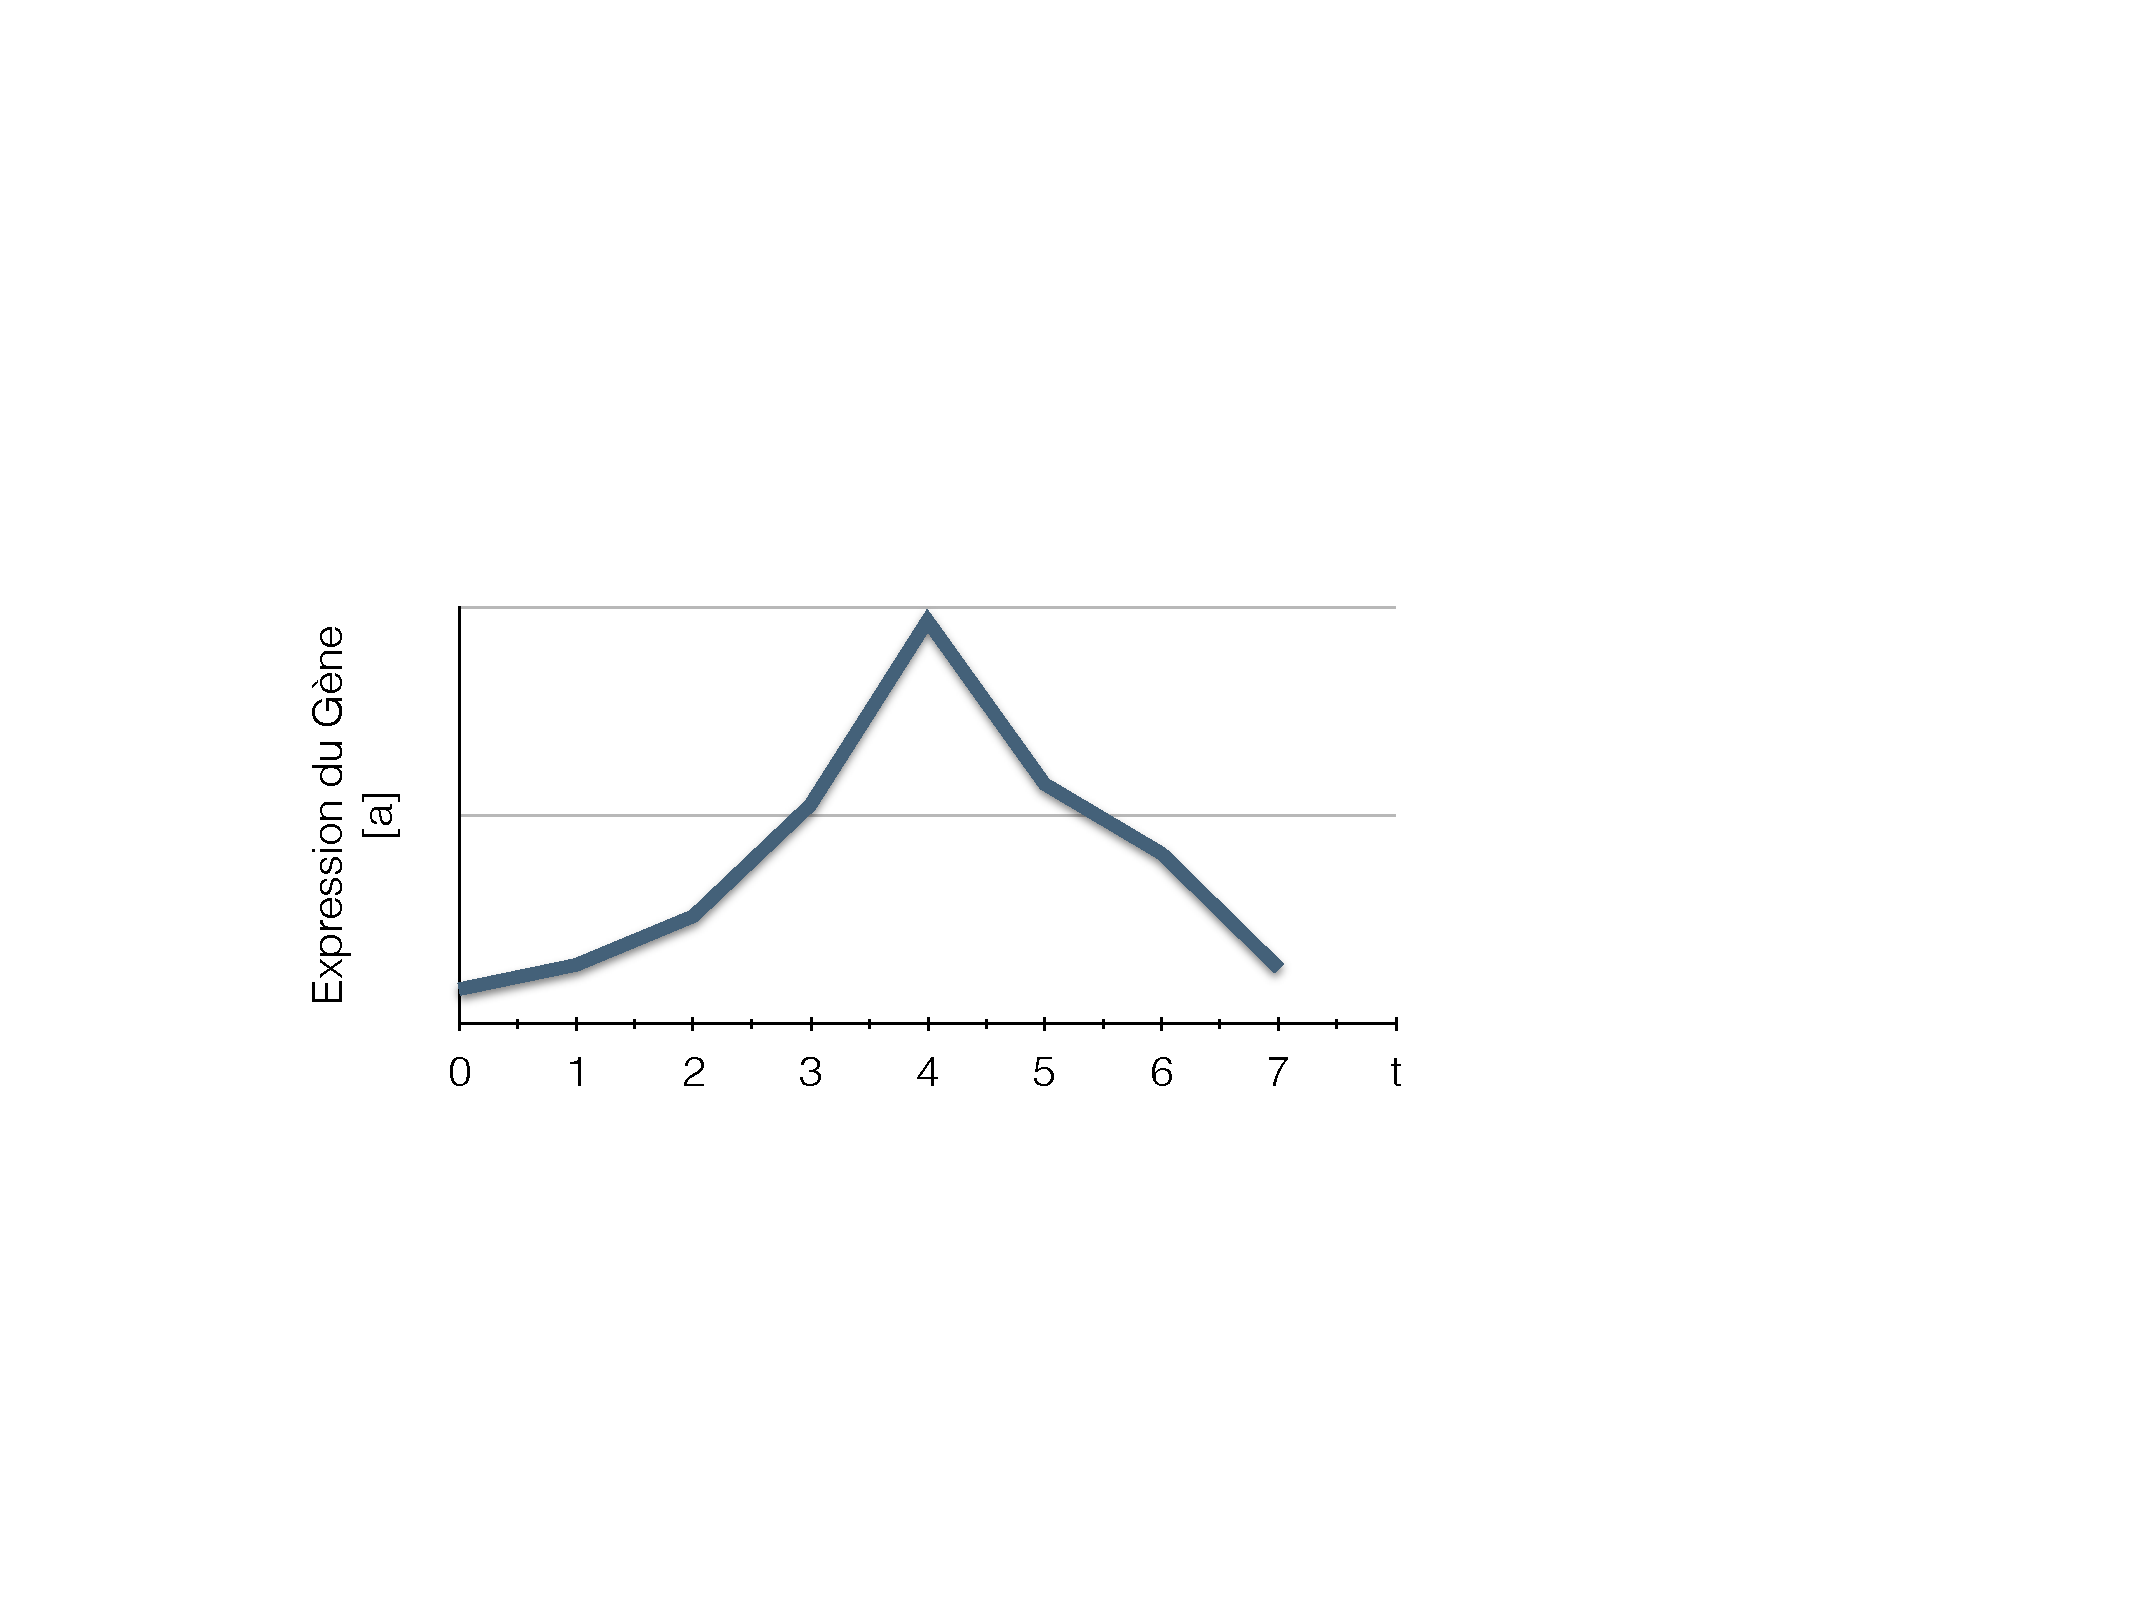
\includegraphics[ width =0.35\linewidth]{images/courbes/gene-a.pdf}\\
%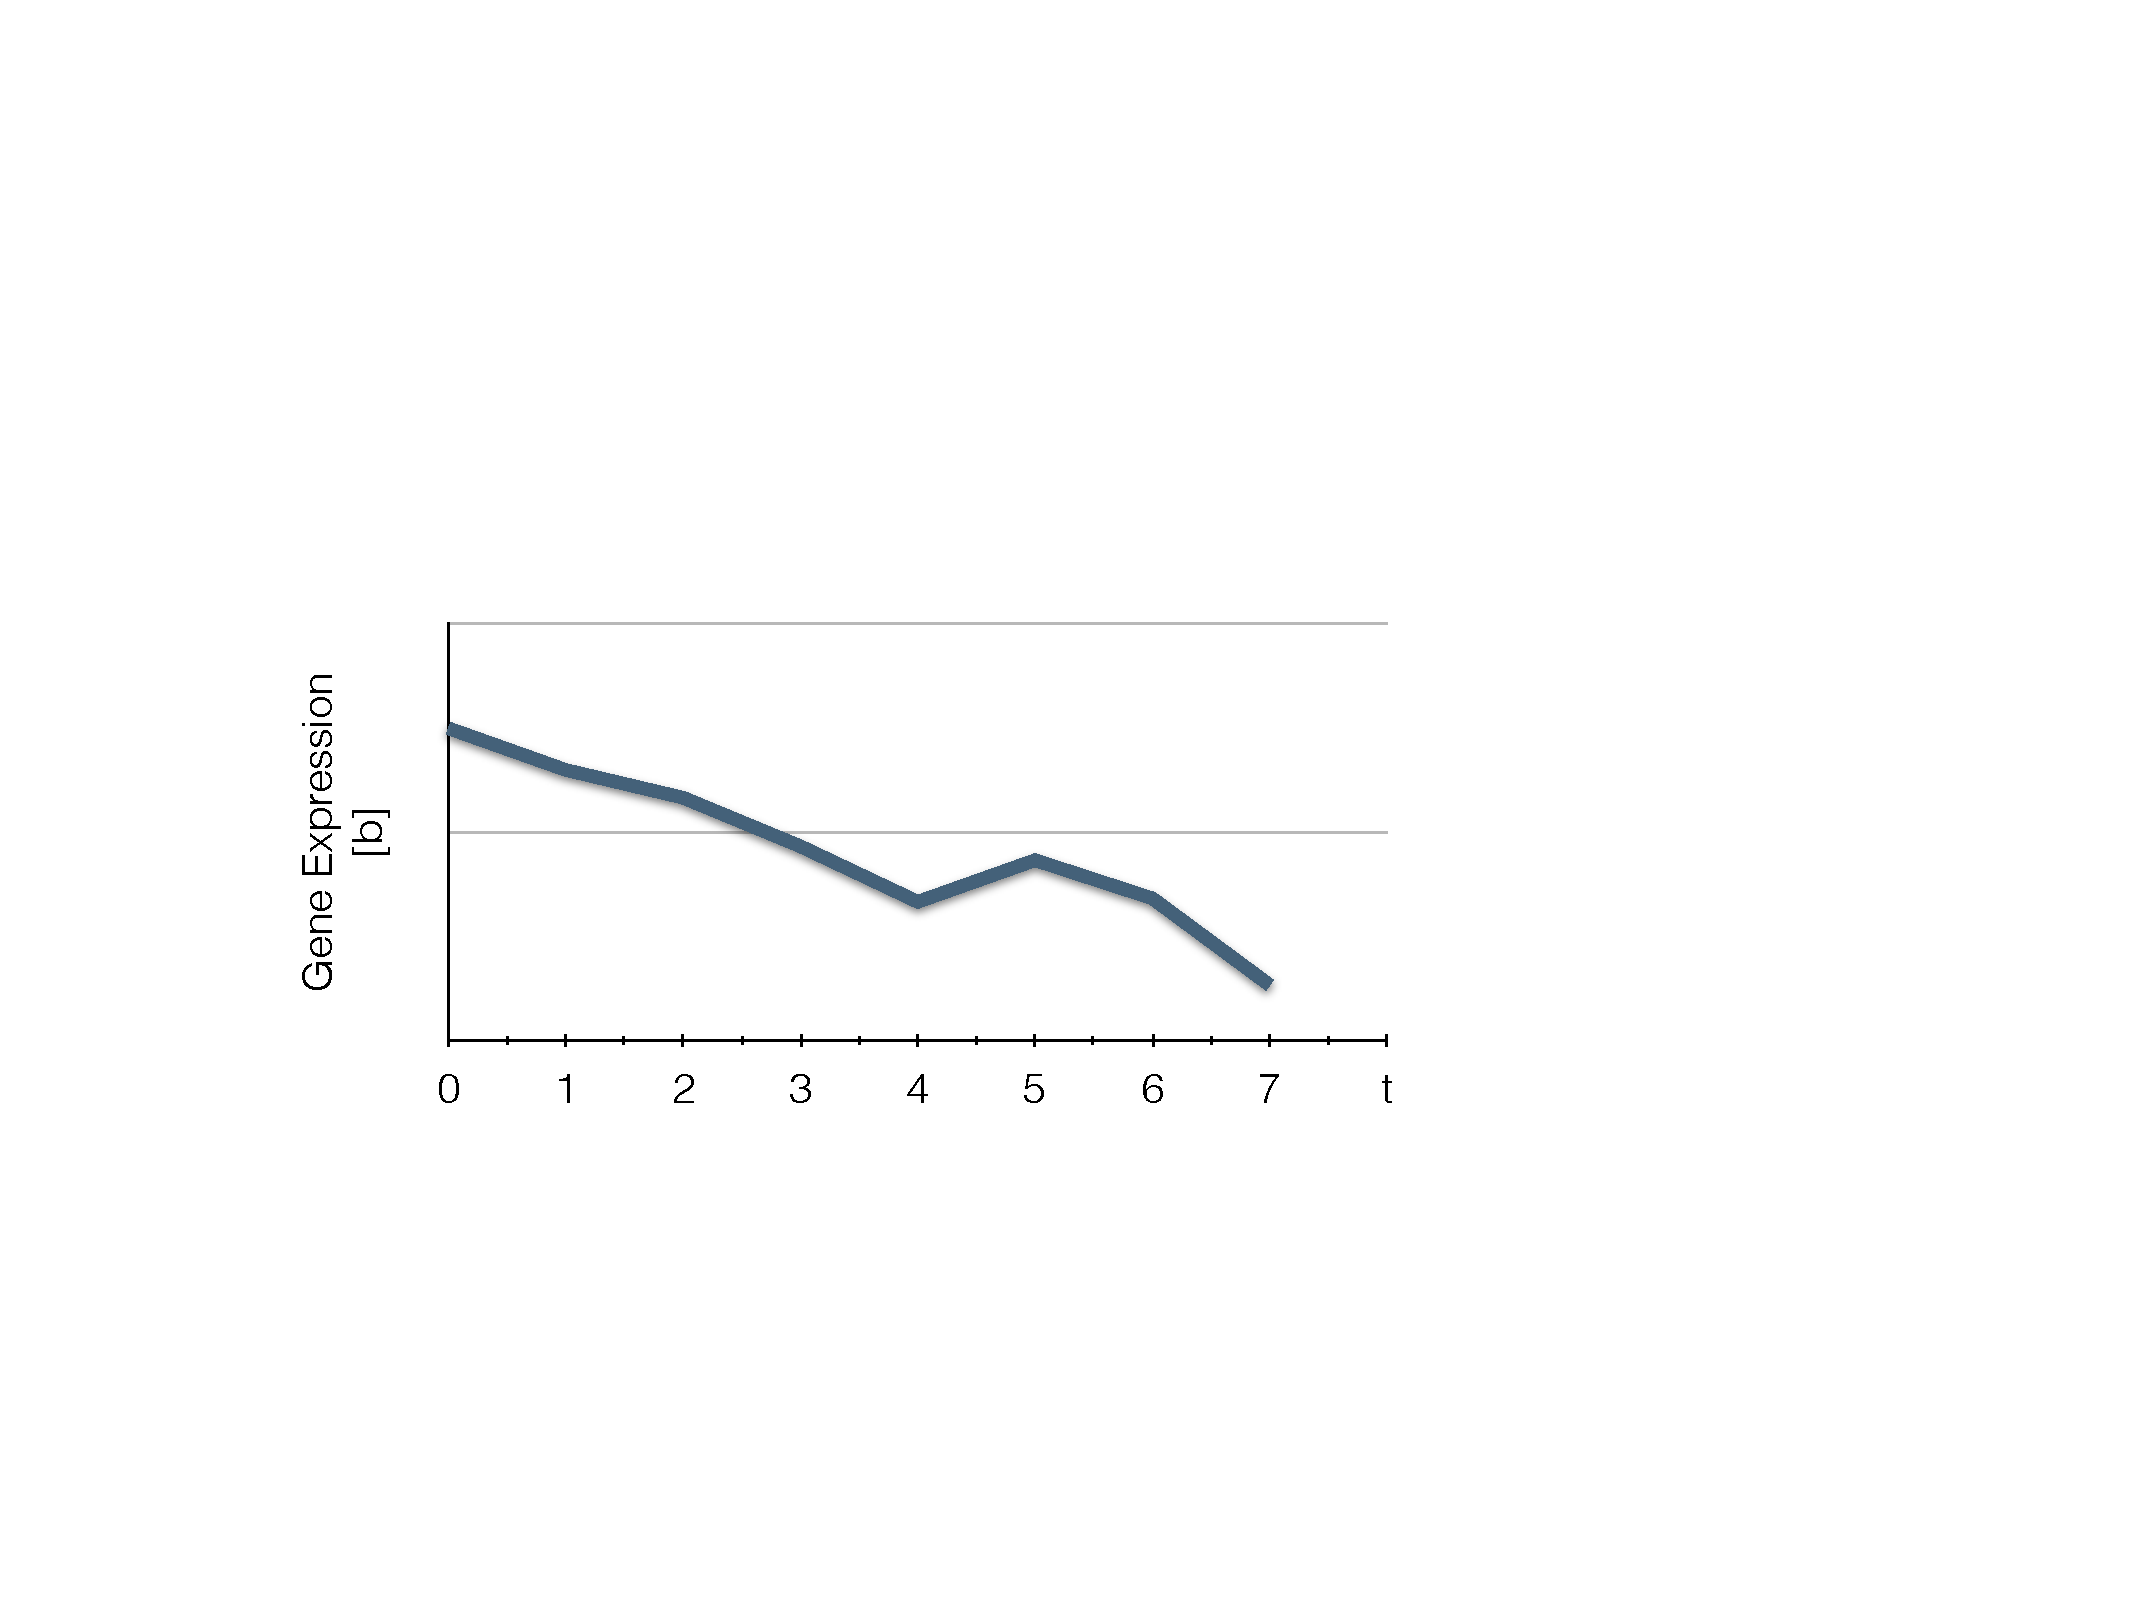
\includegraphics[ width =0.35\linewidth]{images/courbes/gene-b.pdf}\\
%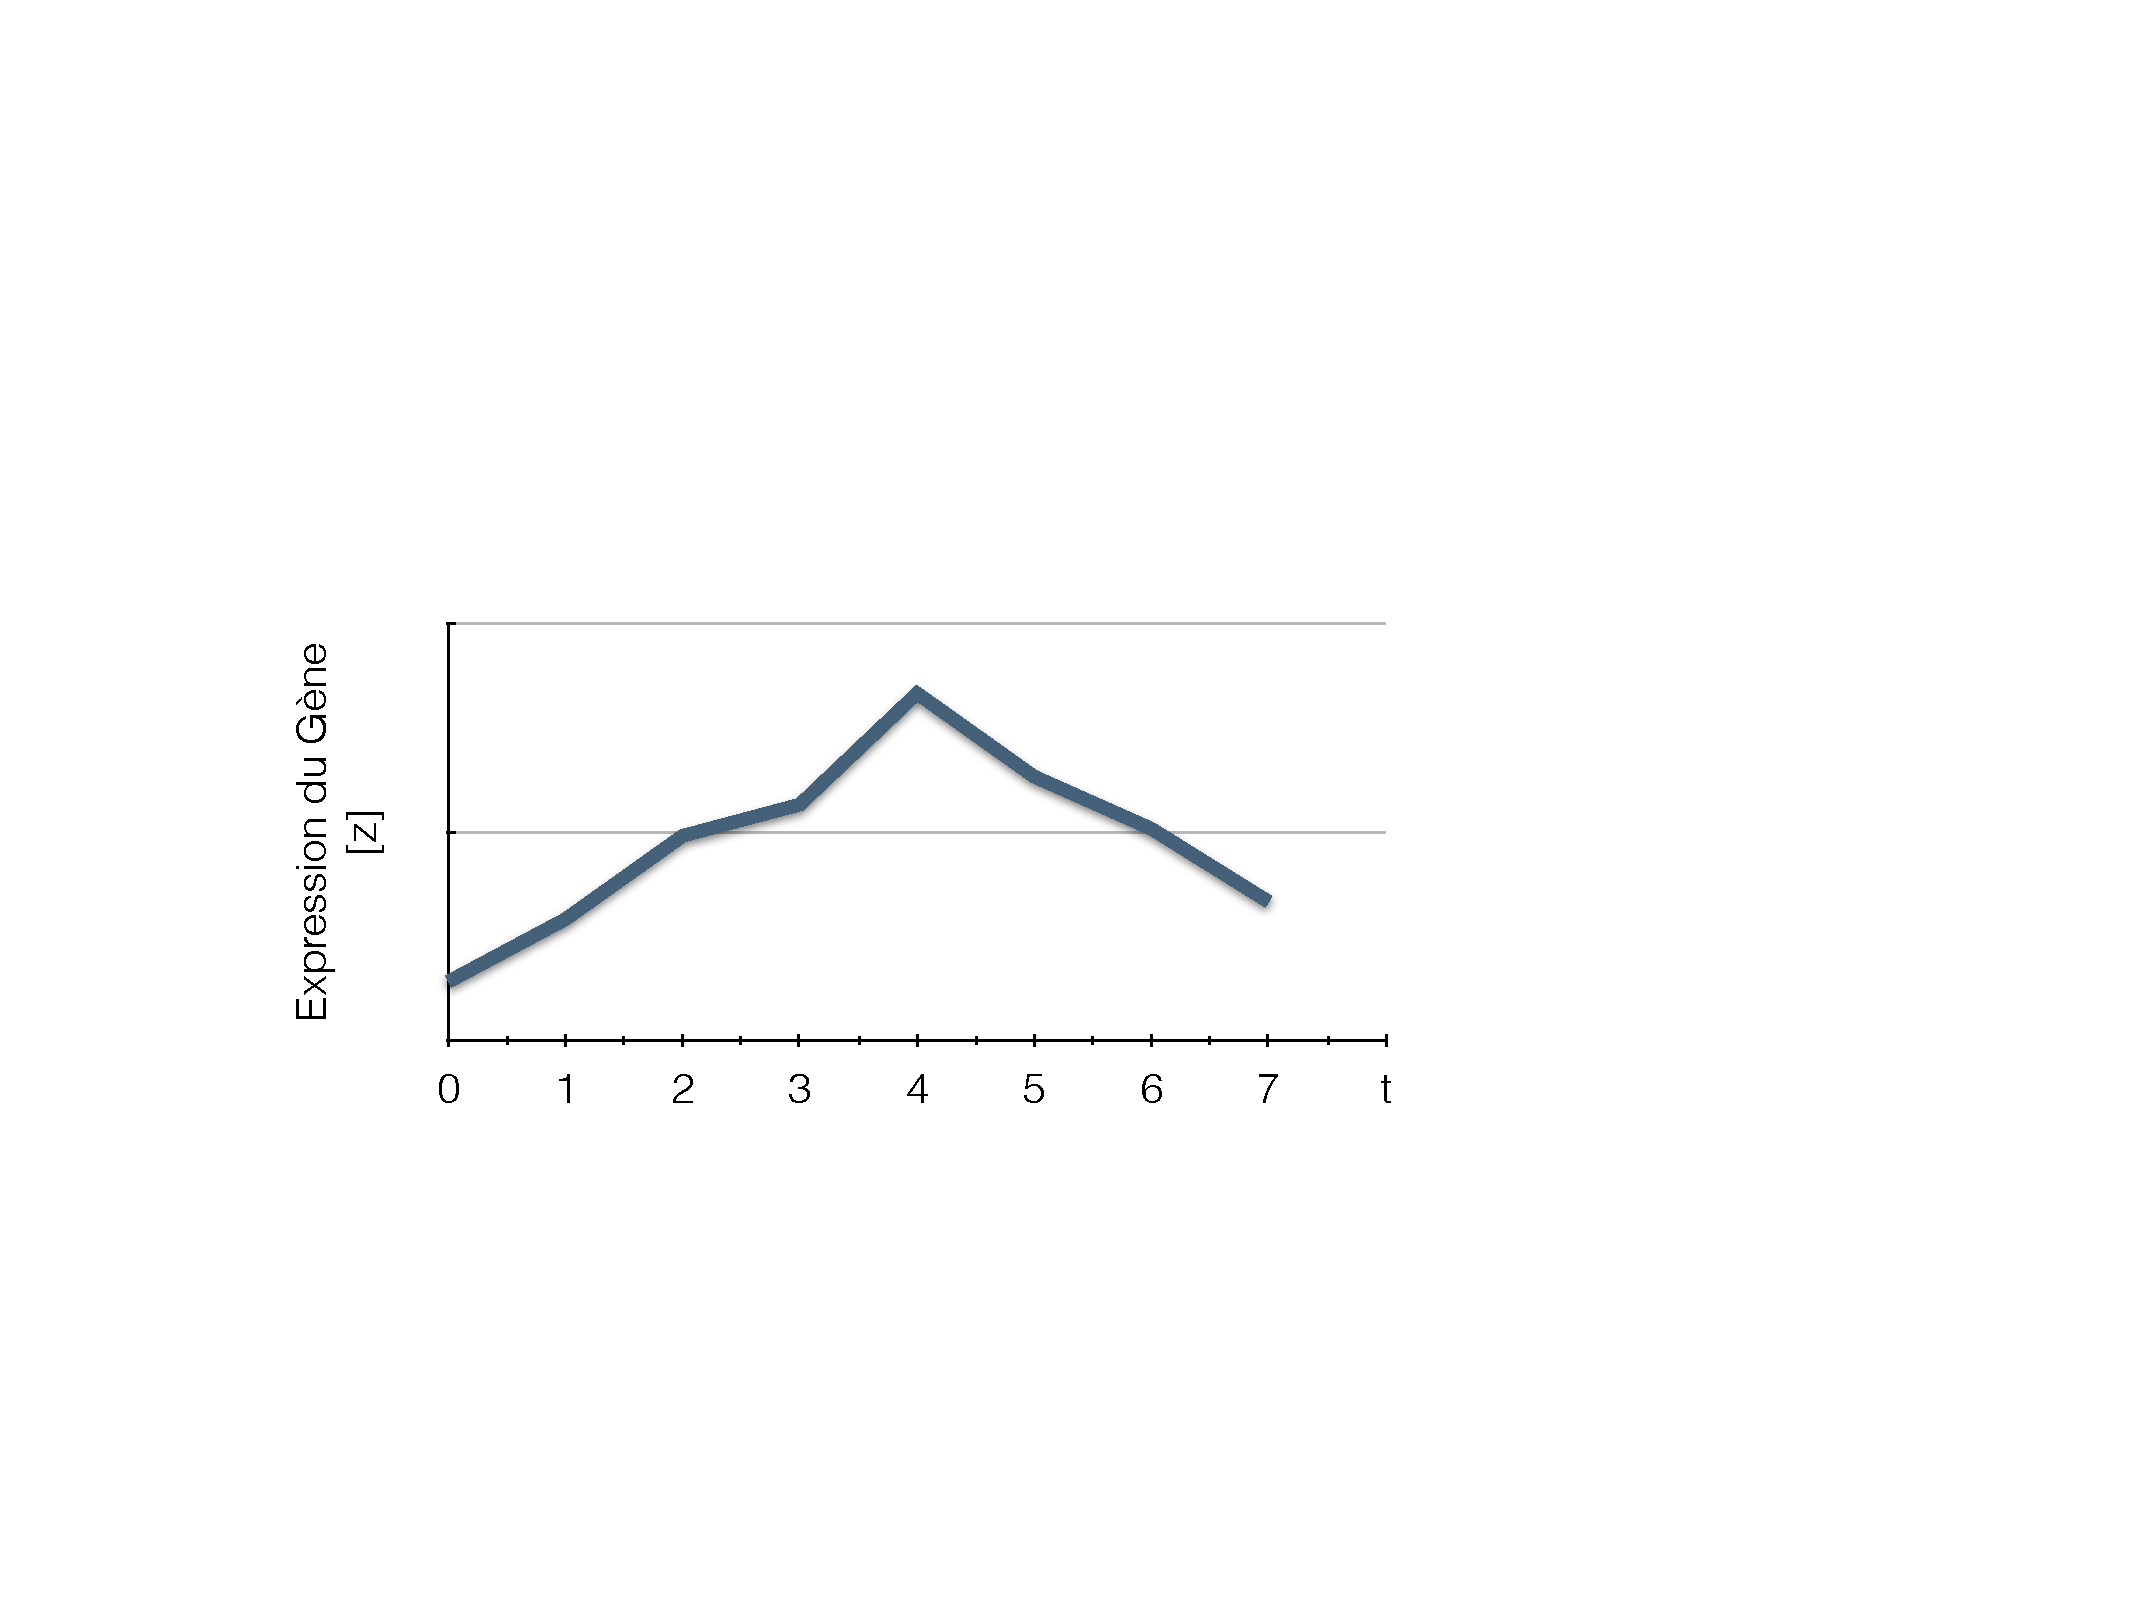
\includegraphics[ width =0.35\linewidth]{images/courbes/gene-z.pdf}
%\hspace{0.01cm}
%\textcolor{red}{$\Rightarrow$}
%\hspace{0.01cm}
%\begin{minipage}[t]{0.4\linewidth}
%\vspace{-5cm}
%Process Hitting:
%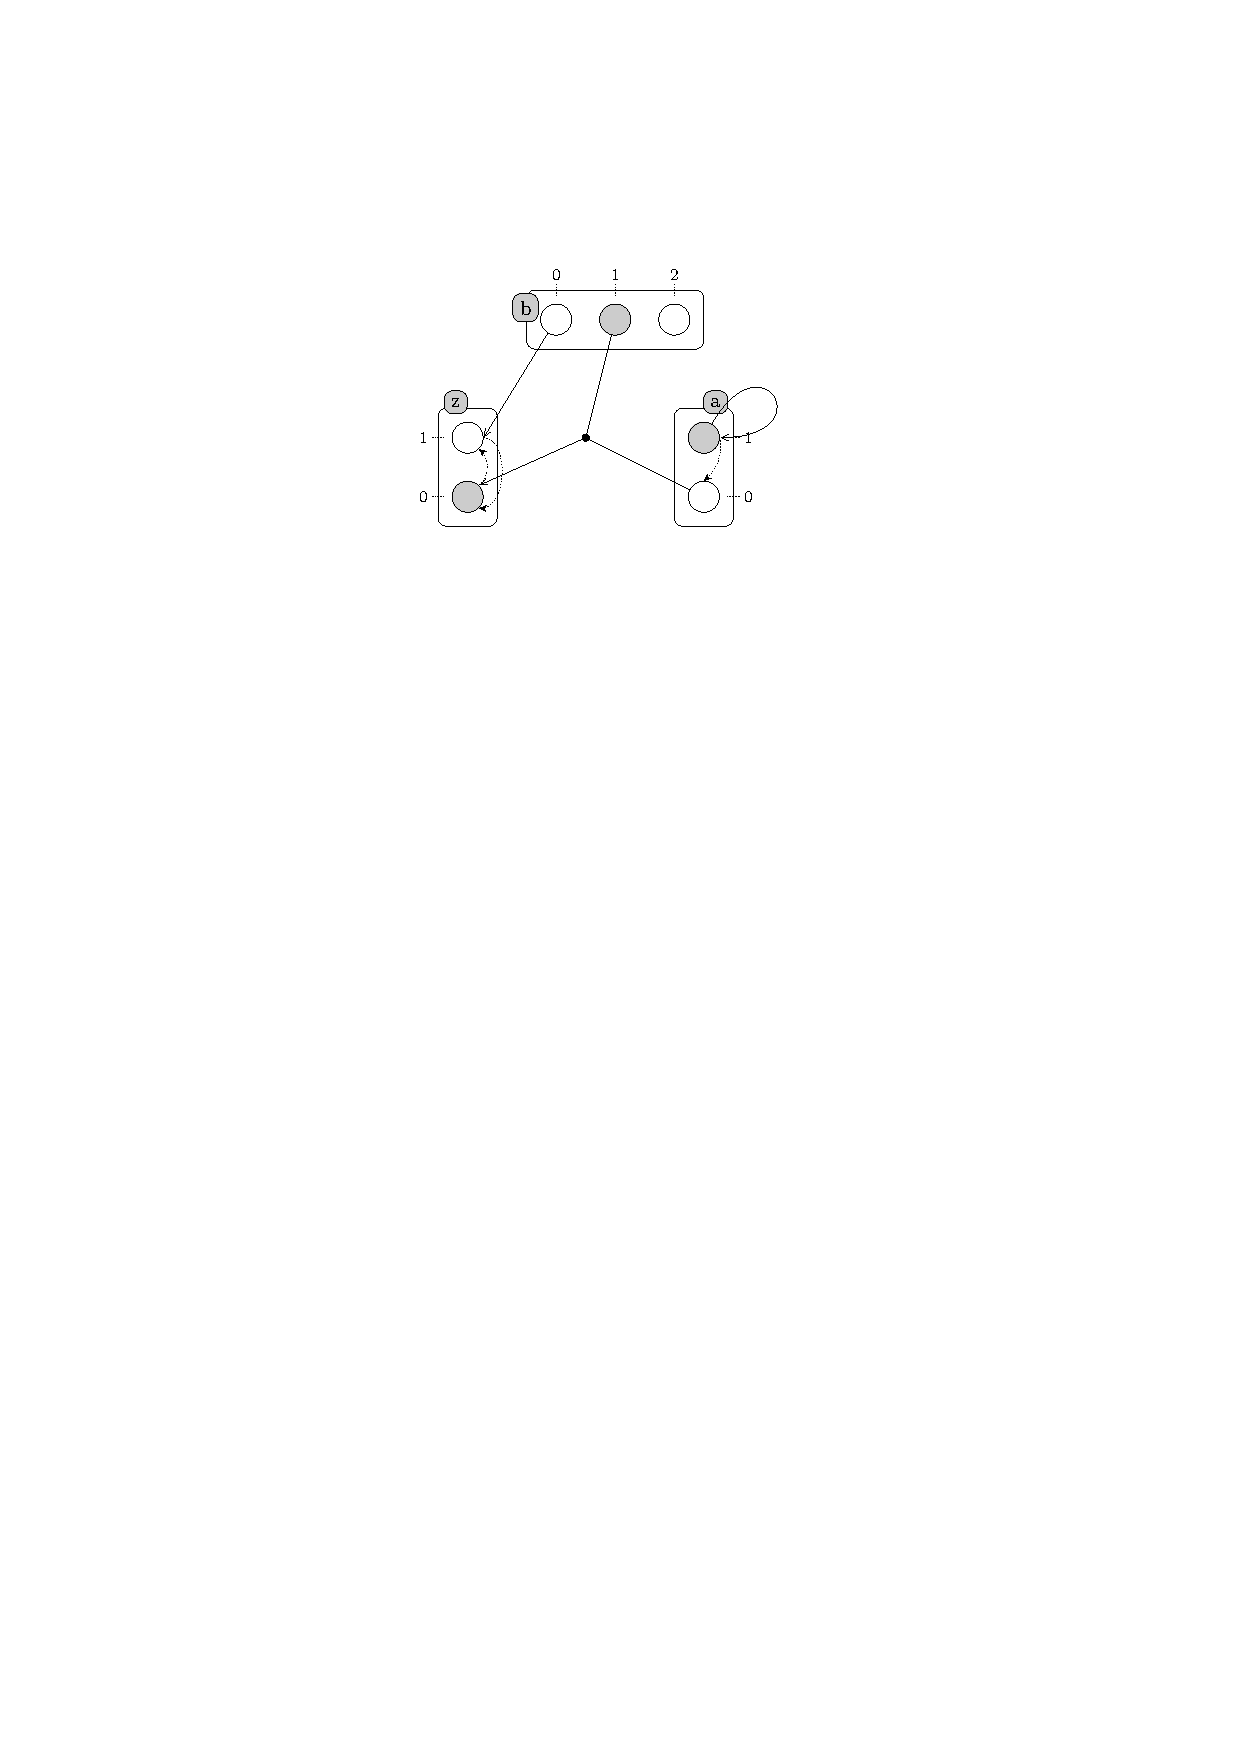
\includegraphics[width =1\linewidth]{images/PH-but.pdf}
%\end{minipage}
%\end{figure}


% Discretization figure
\begin{figure}[h]\centering
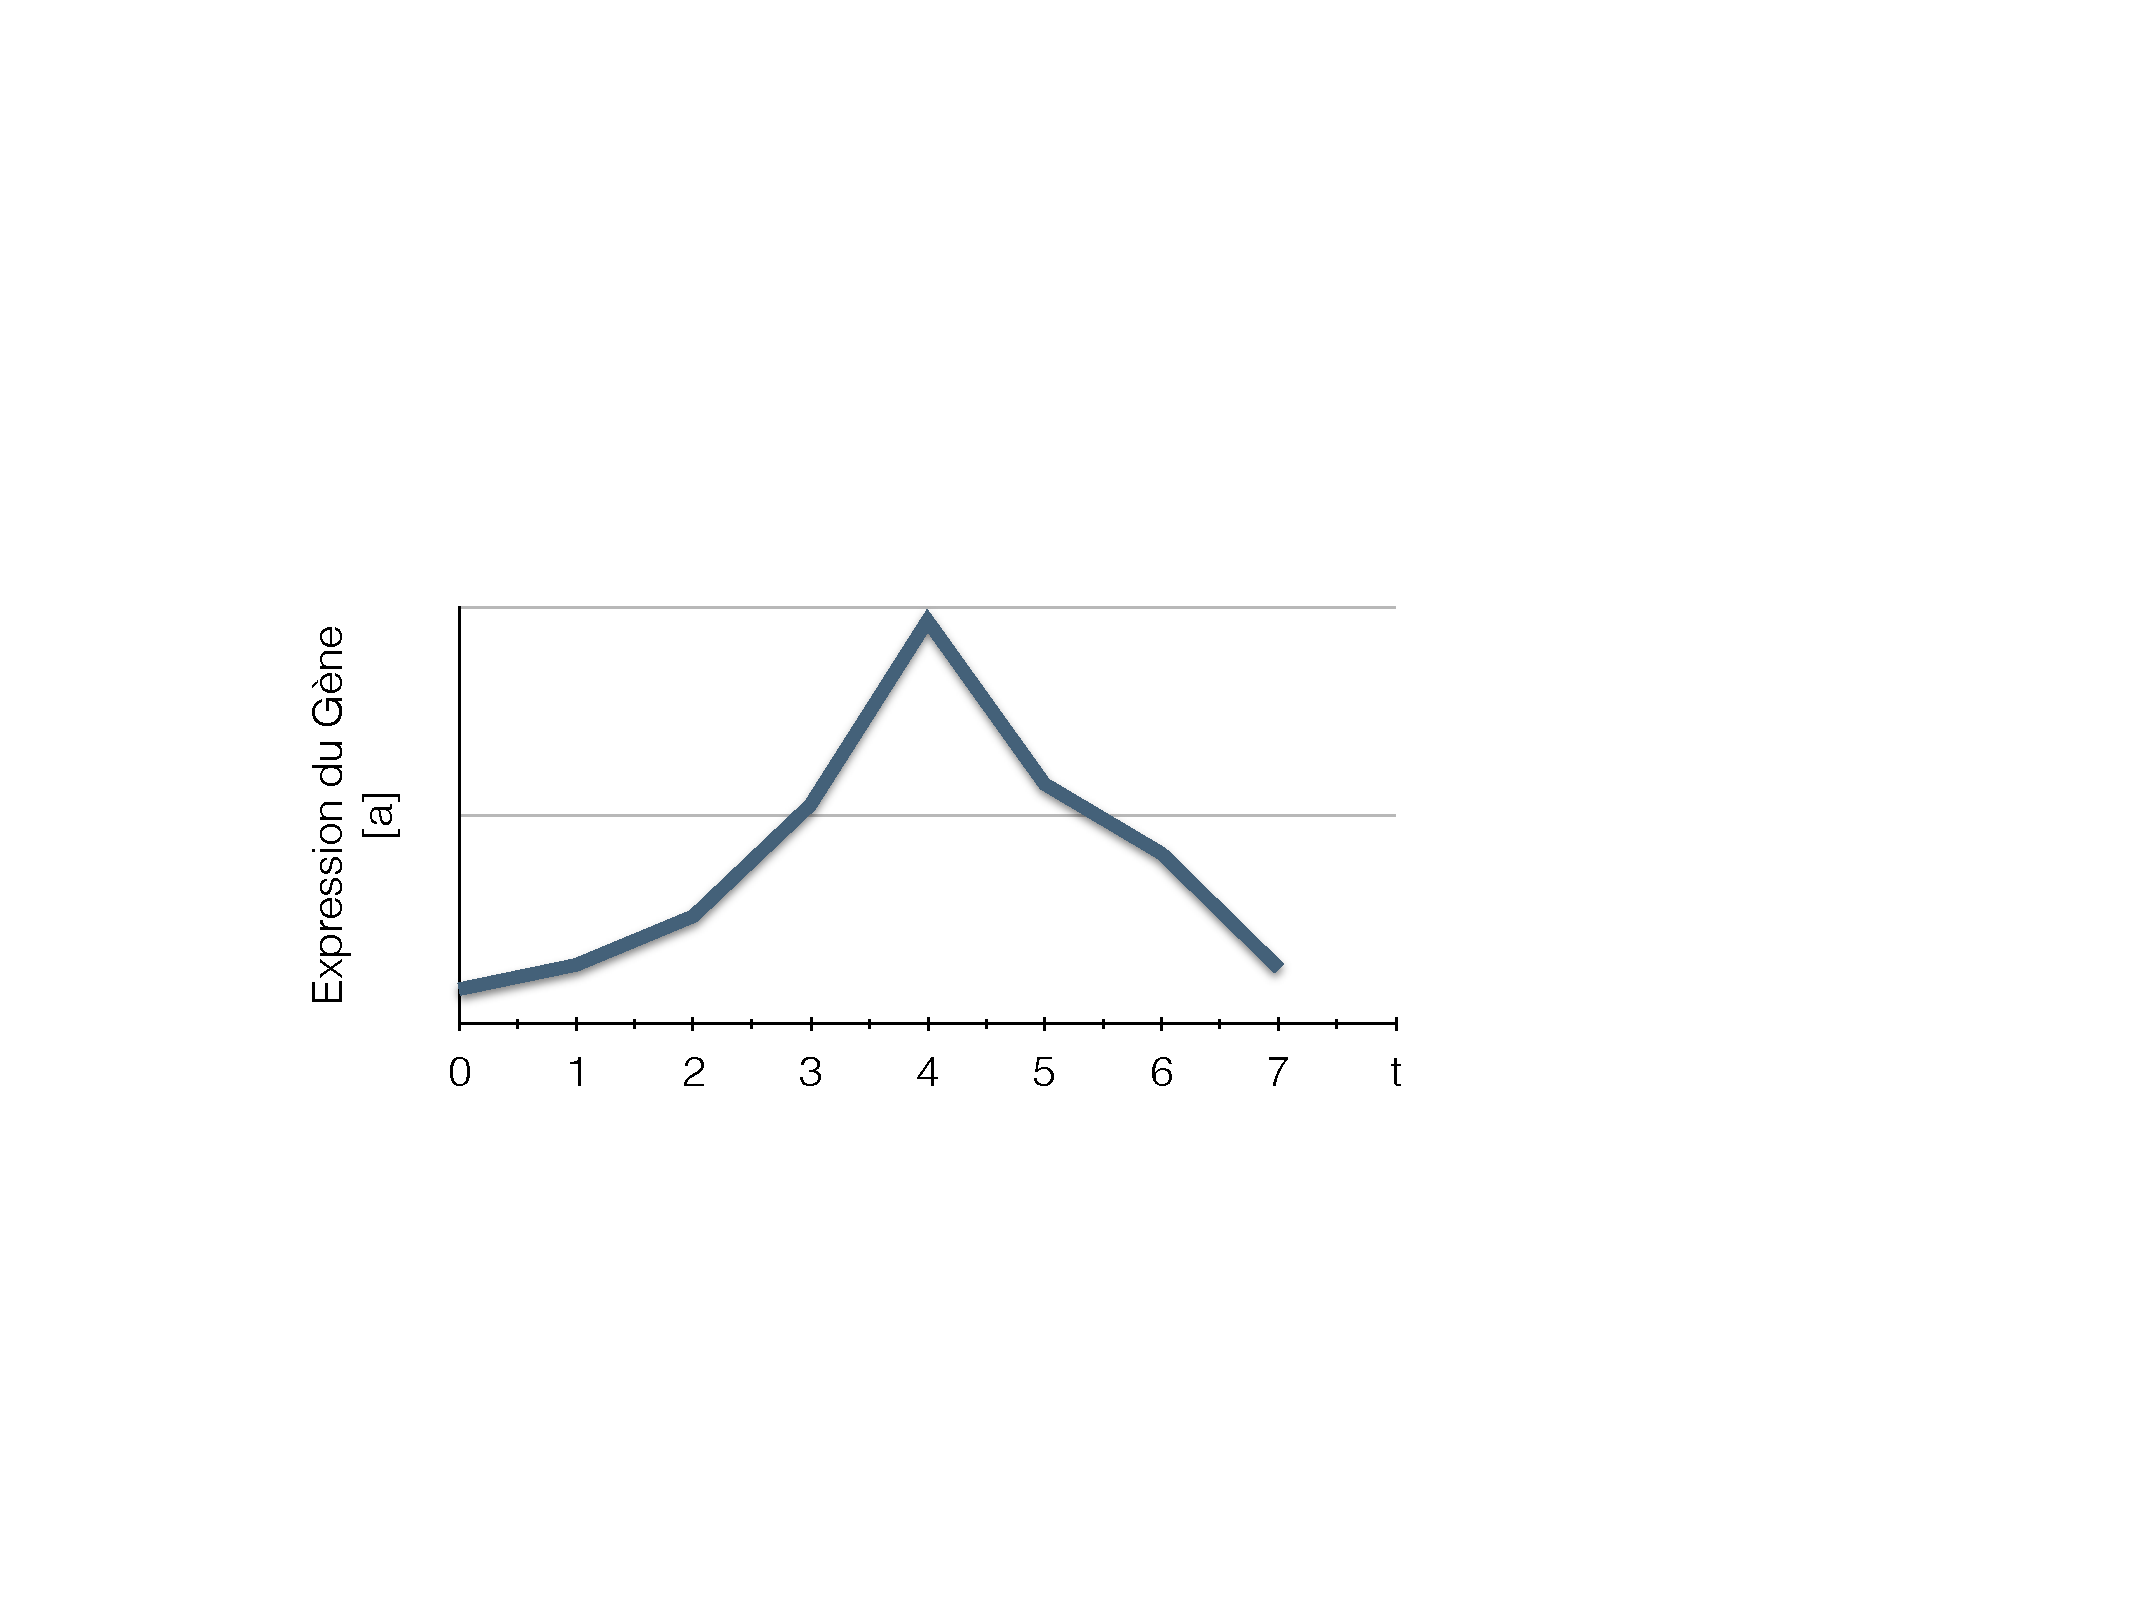
\includegraphics[width =0.31\linewidth]{images/courbes/gene-a.pdf}
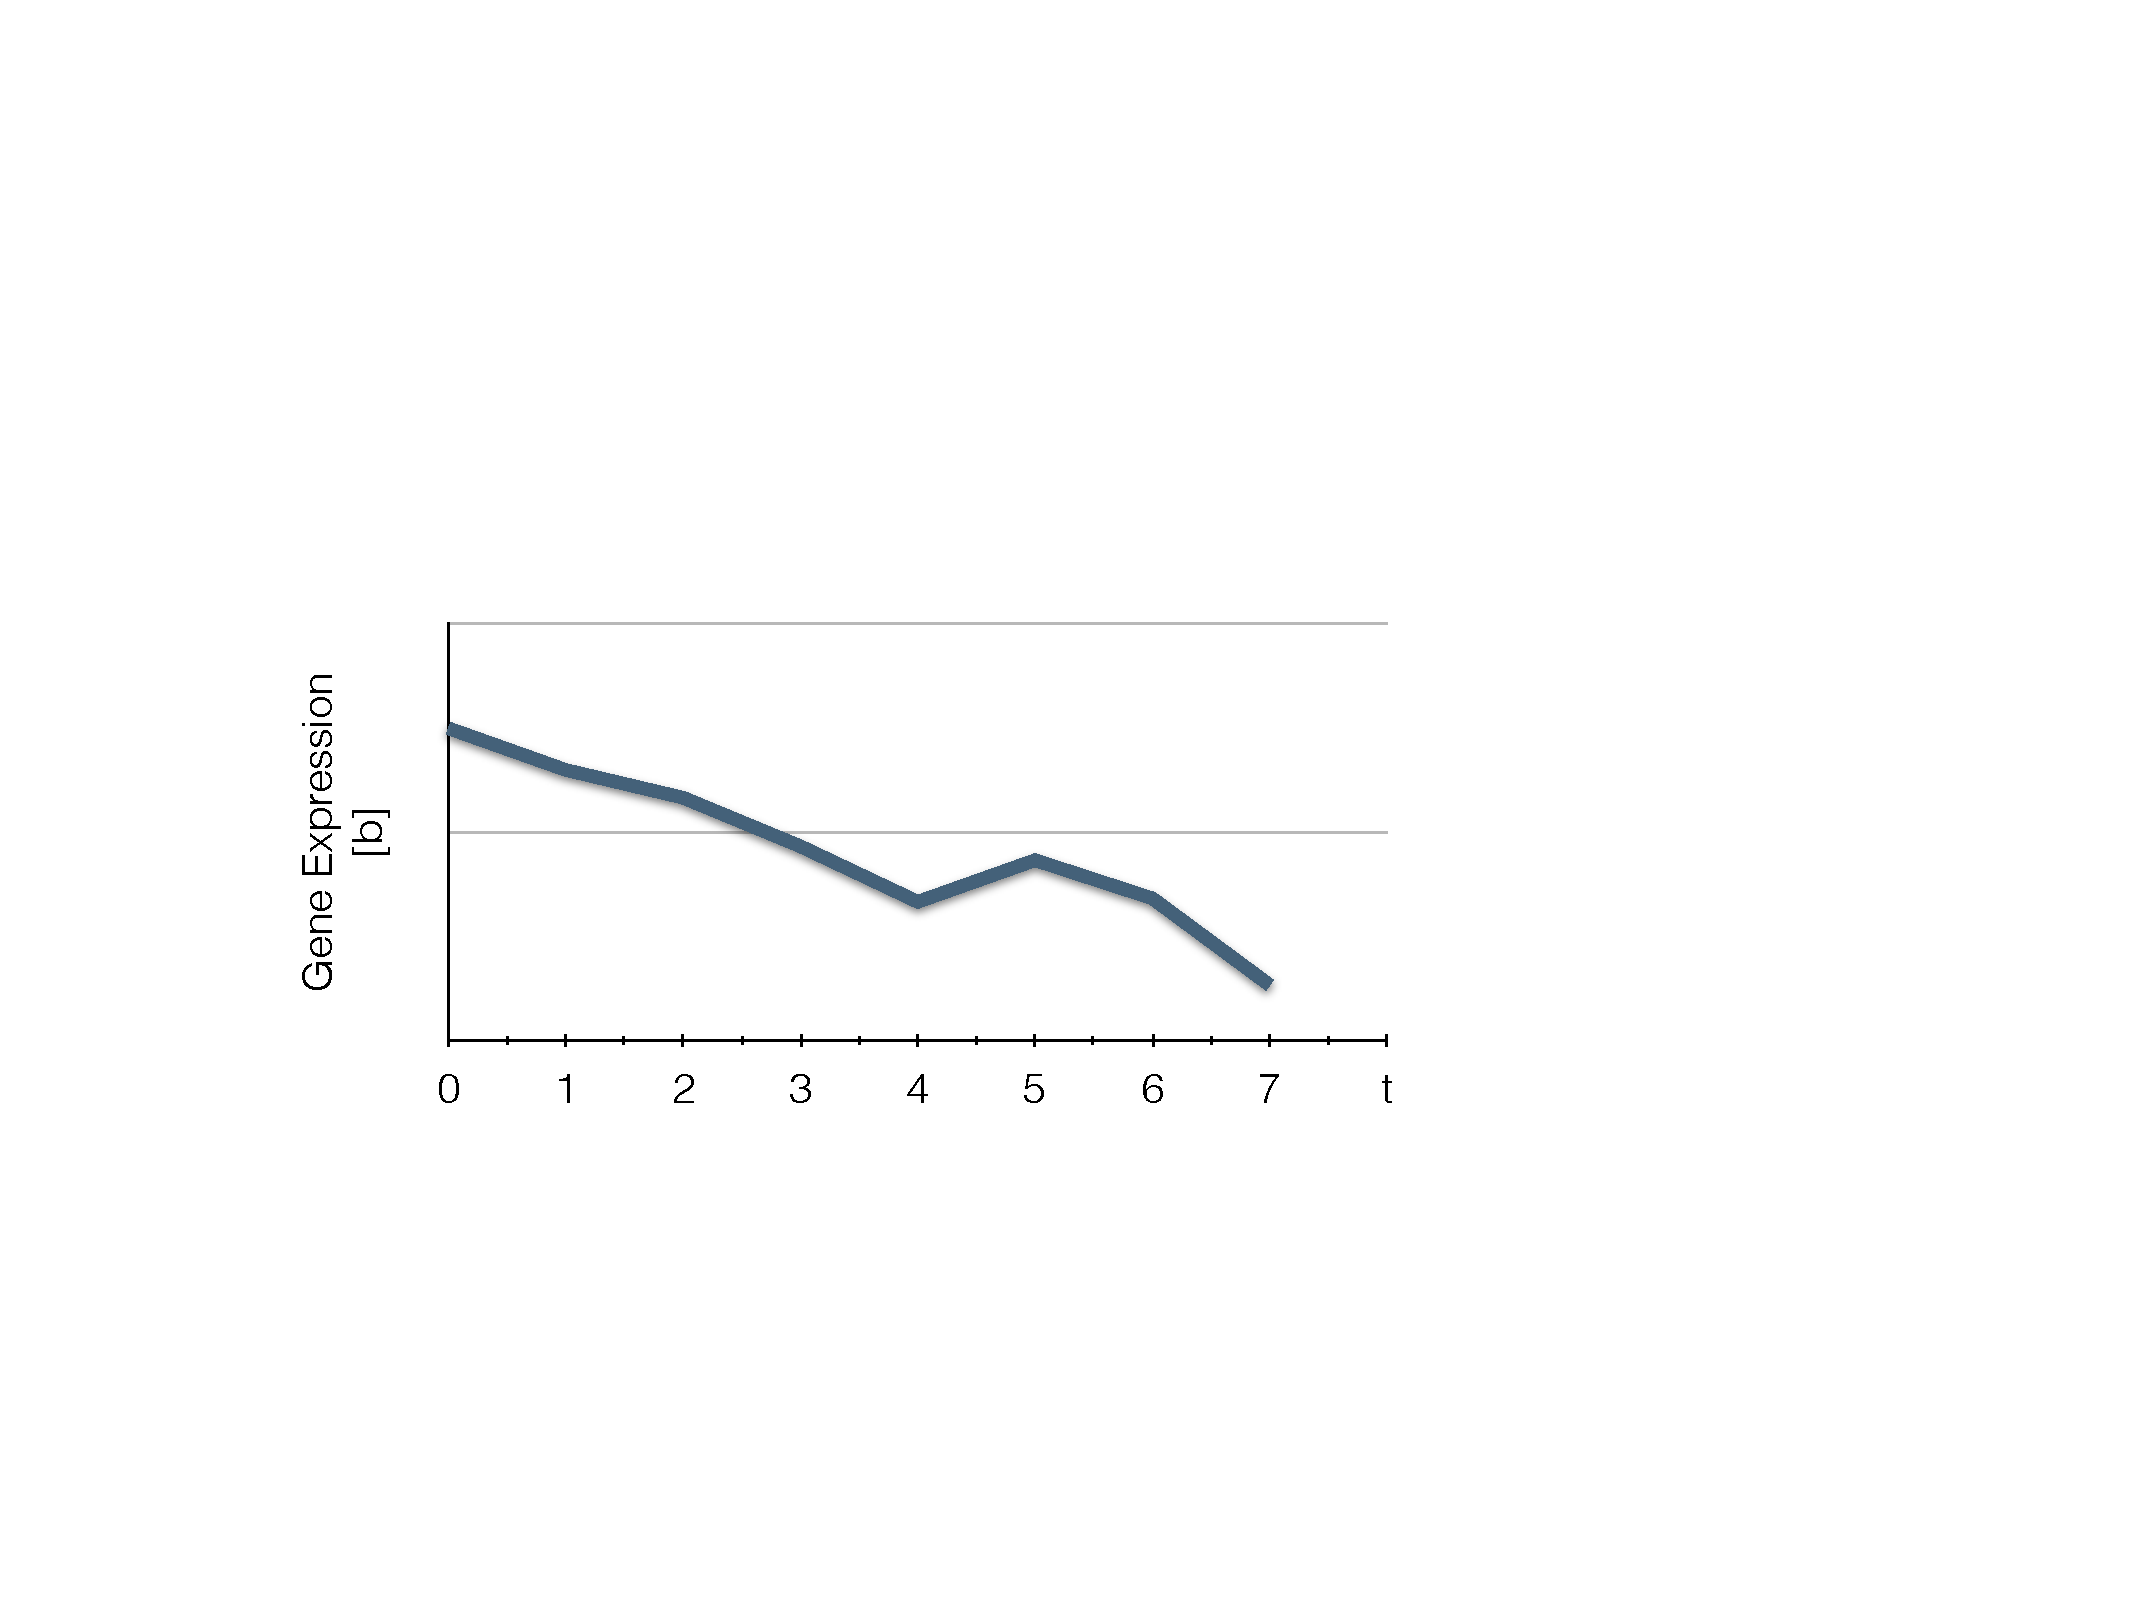
\includegraphics[width =0.31\linewidth]{images/courbes/gene-b.pdf}
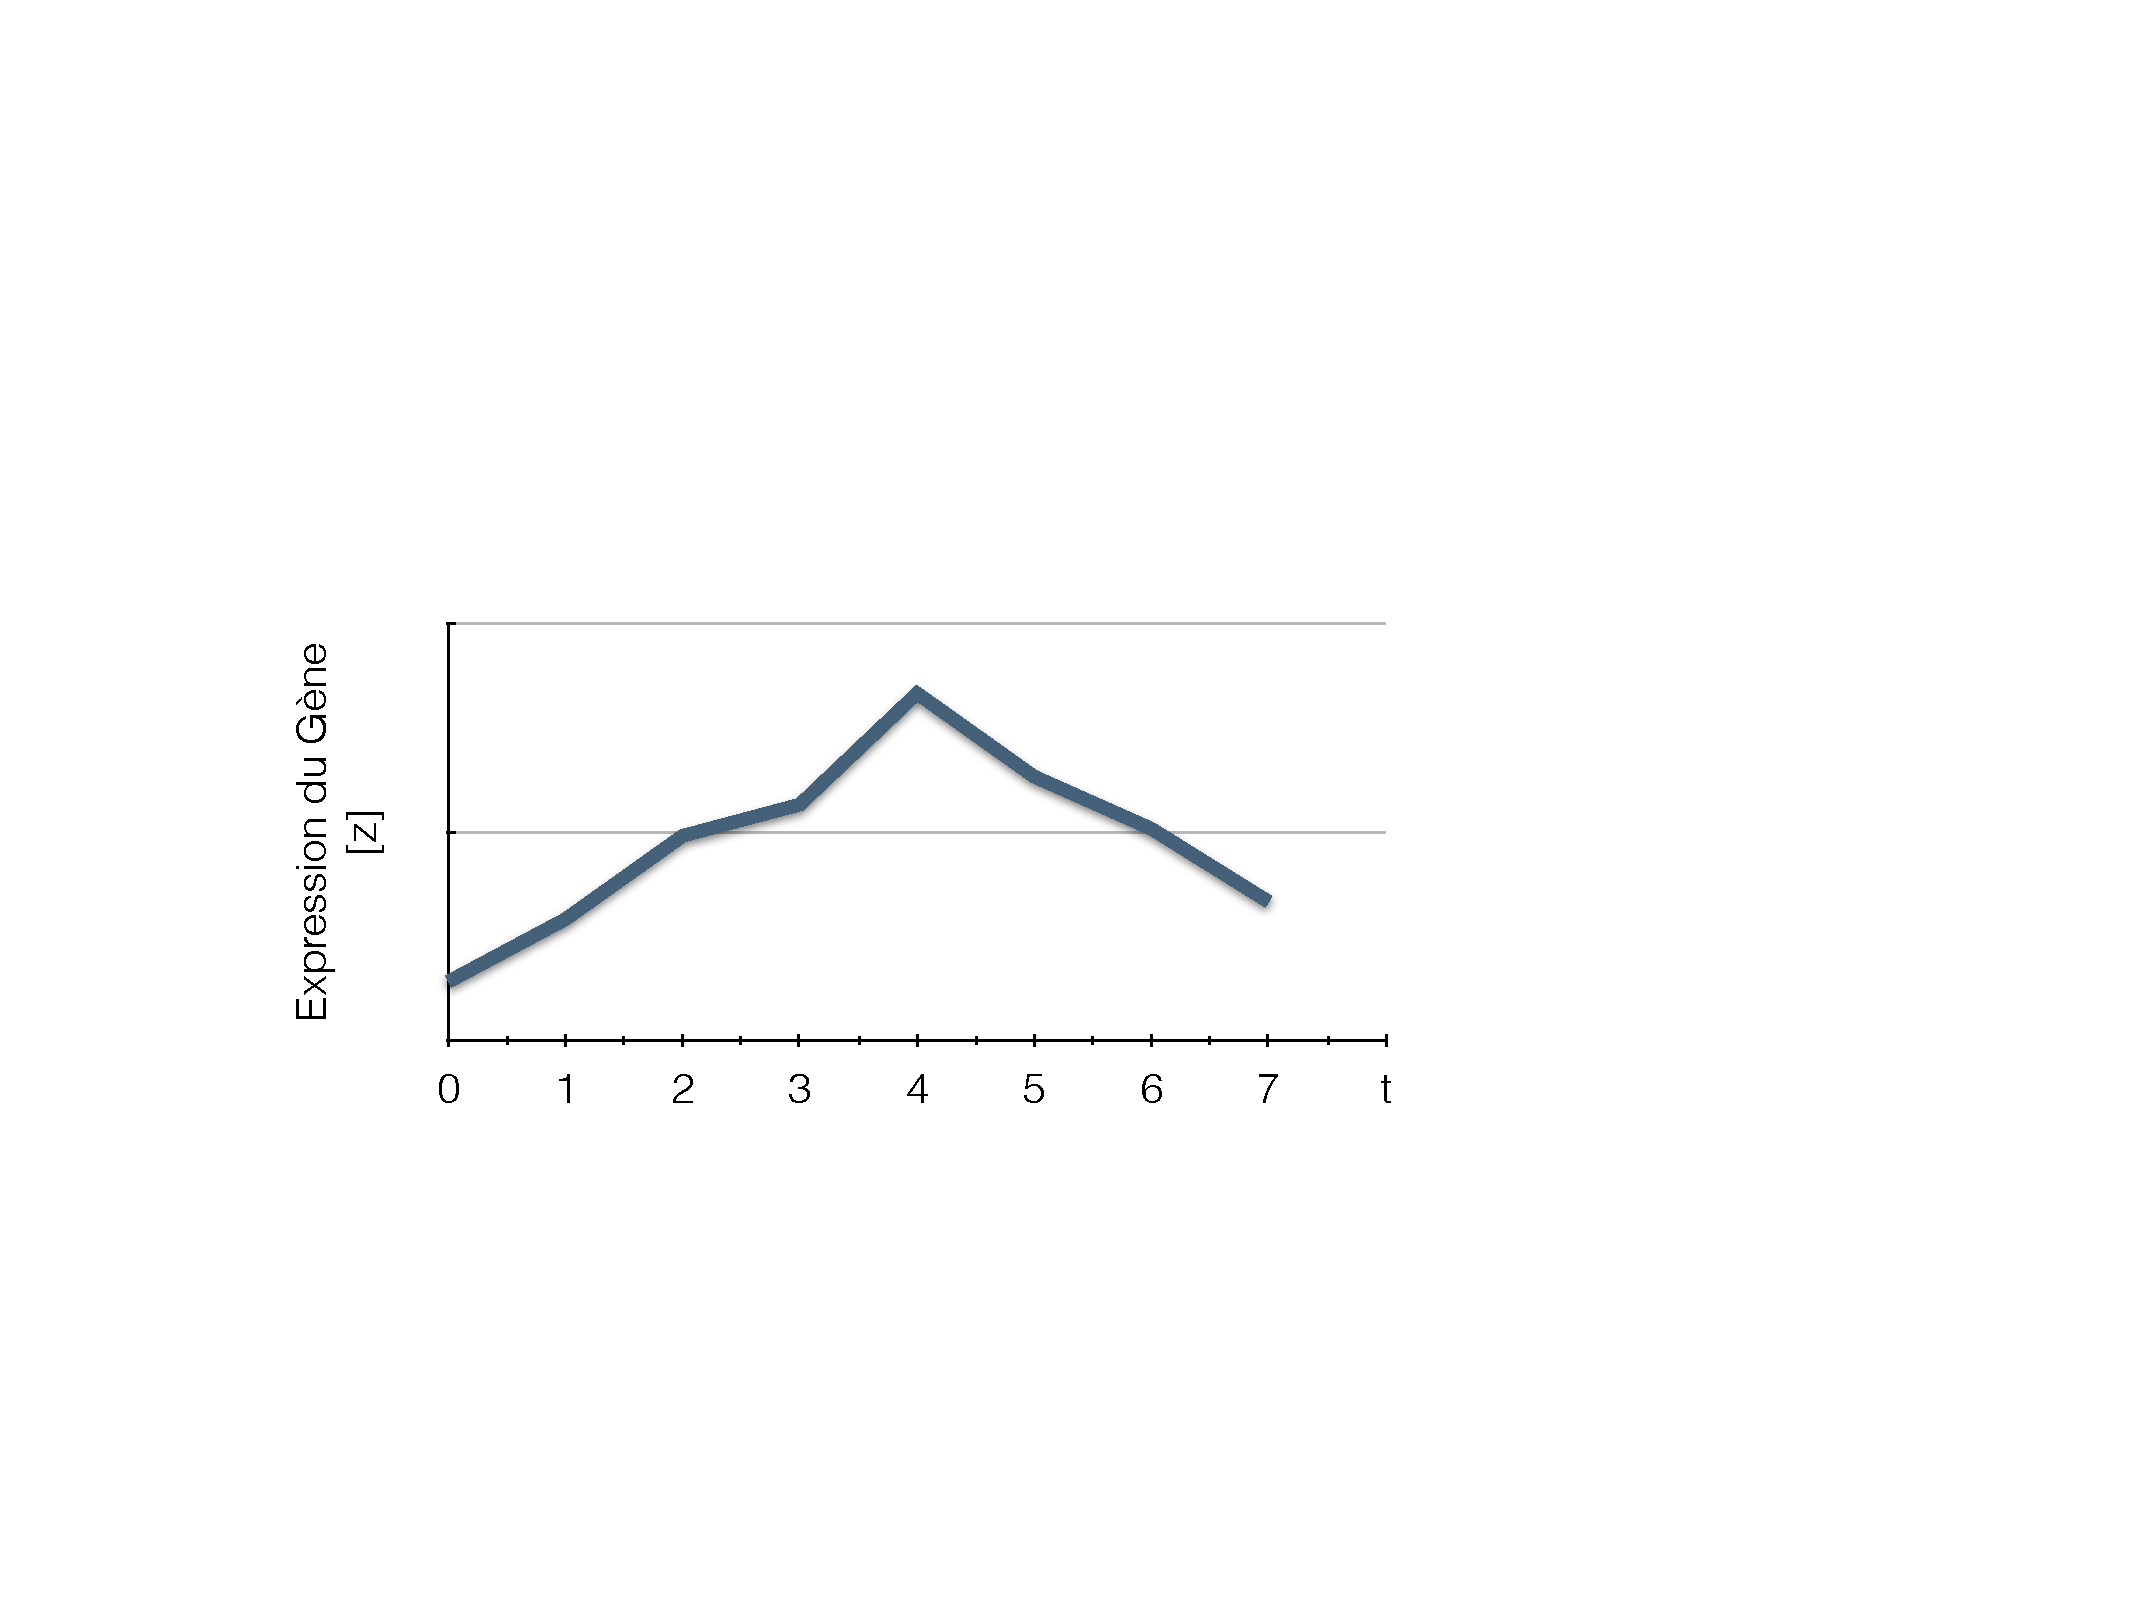
\includegraphics[width =0.31\linewidth]{images/courbes/gene-z.pdf}

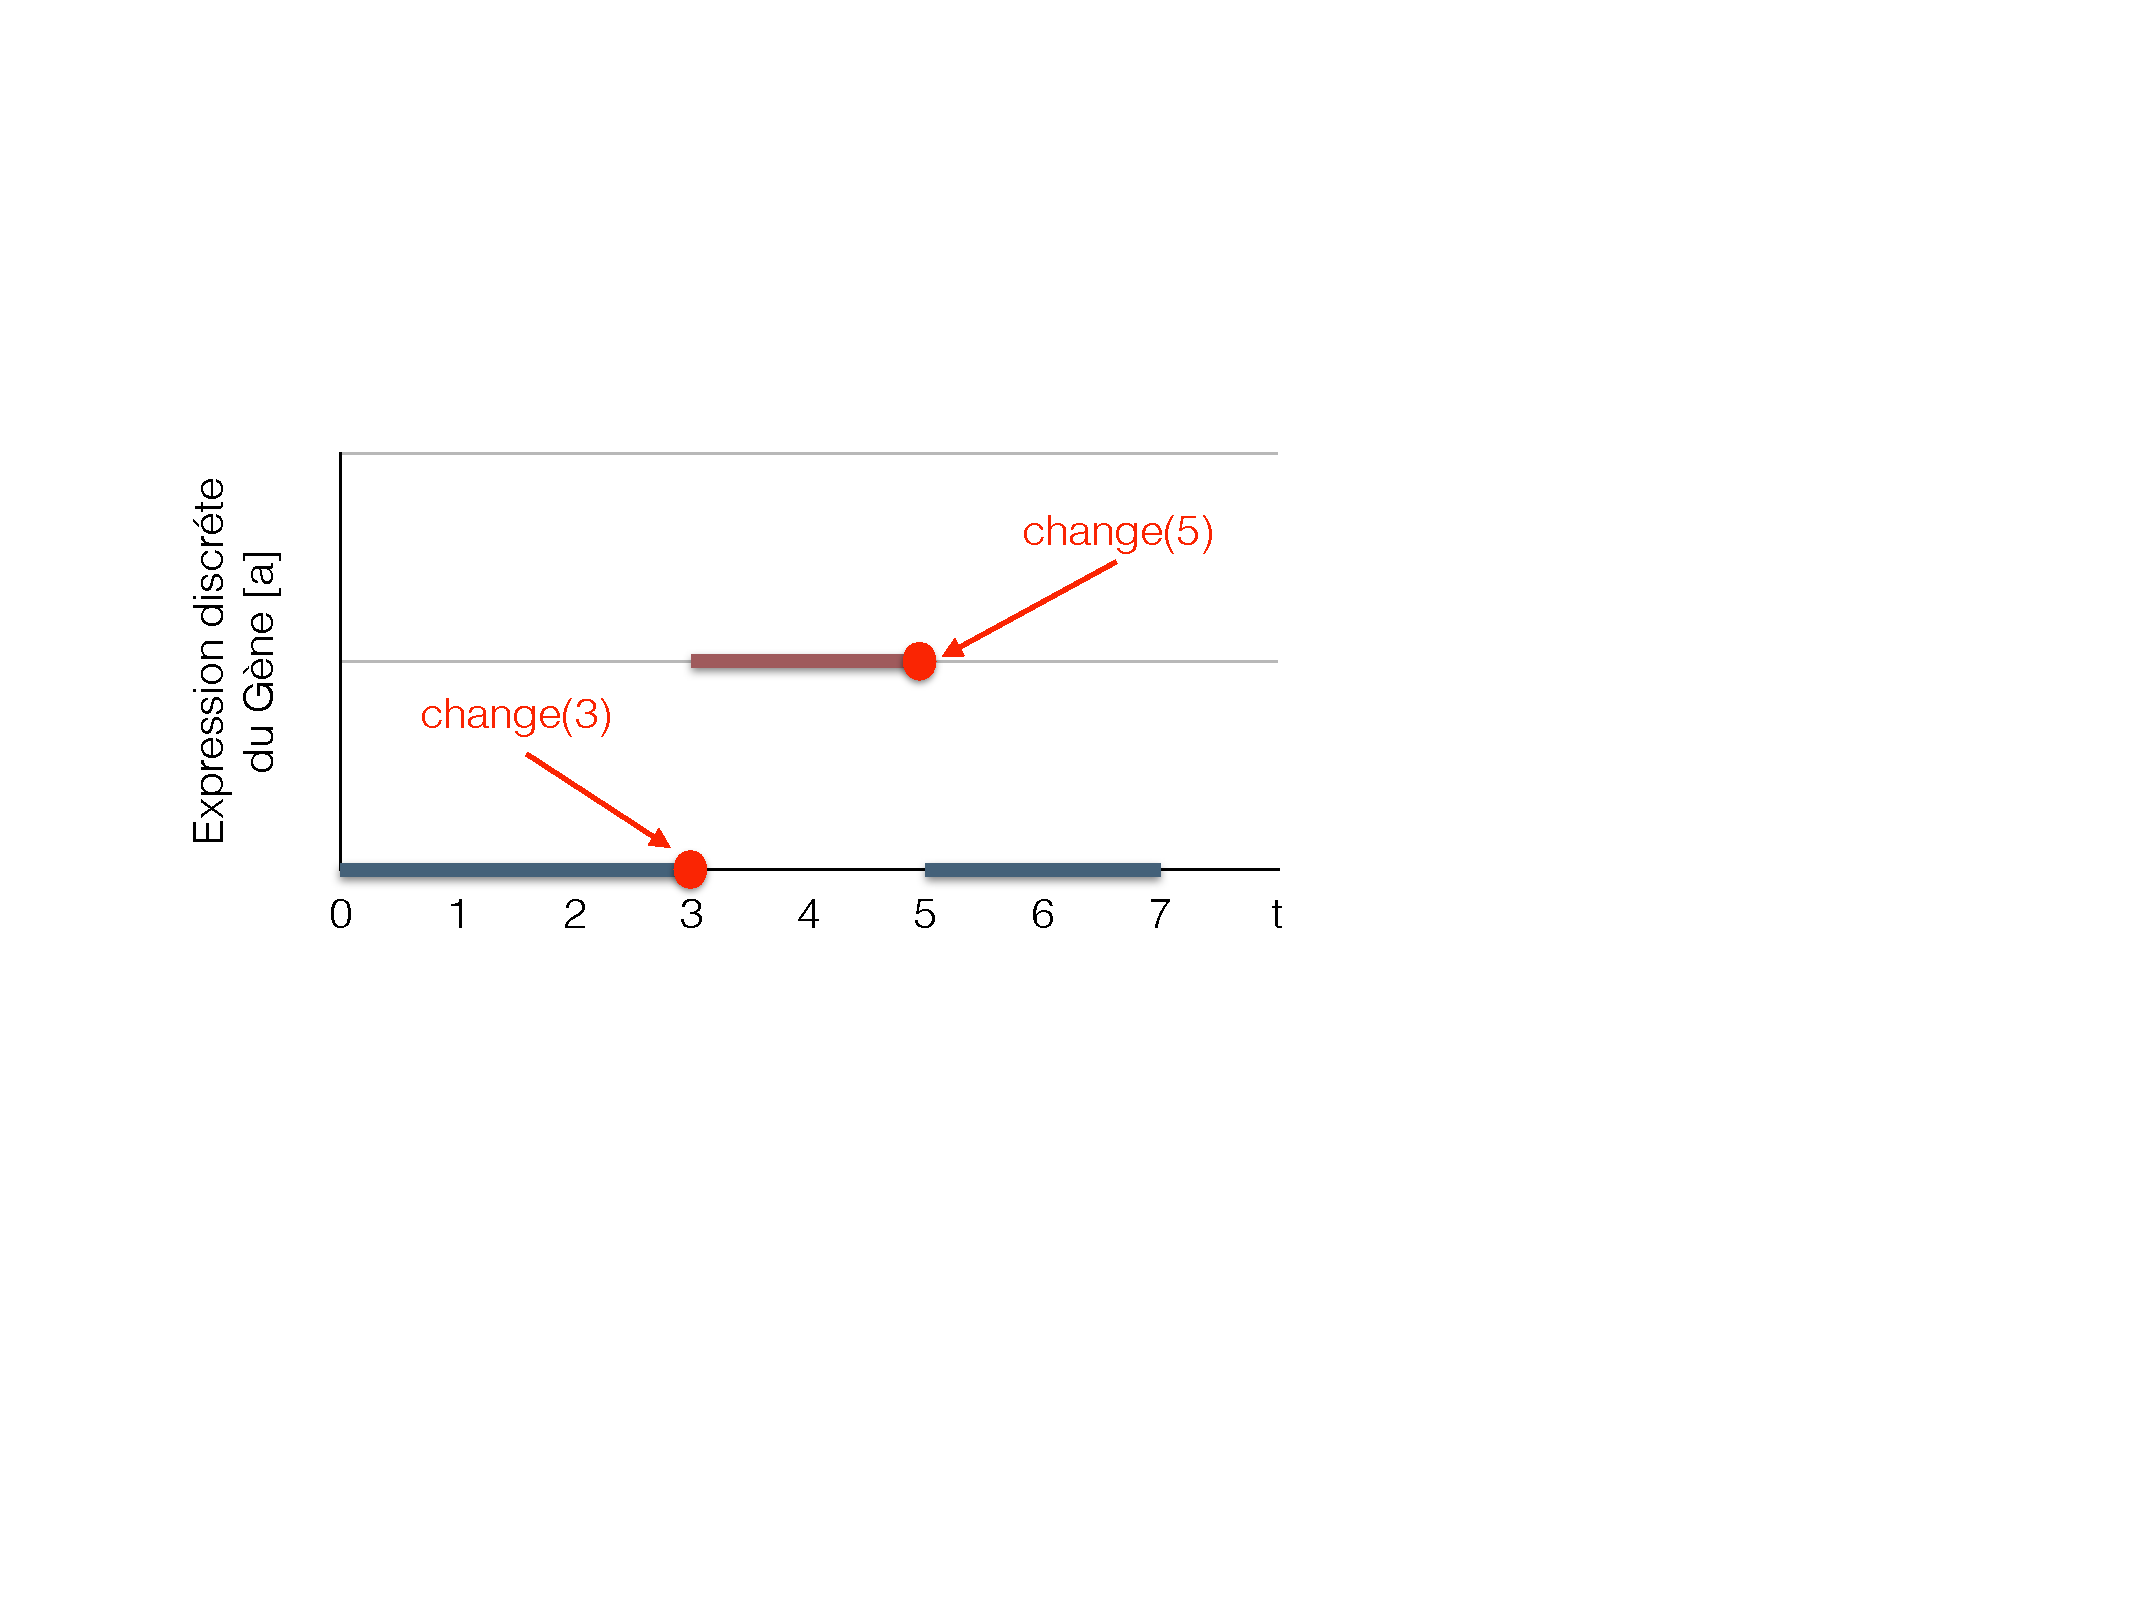
\includegraphics[width =0.31\linewidth]{images/courbes/gene-a-disc-change.pdf}
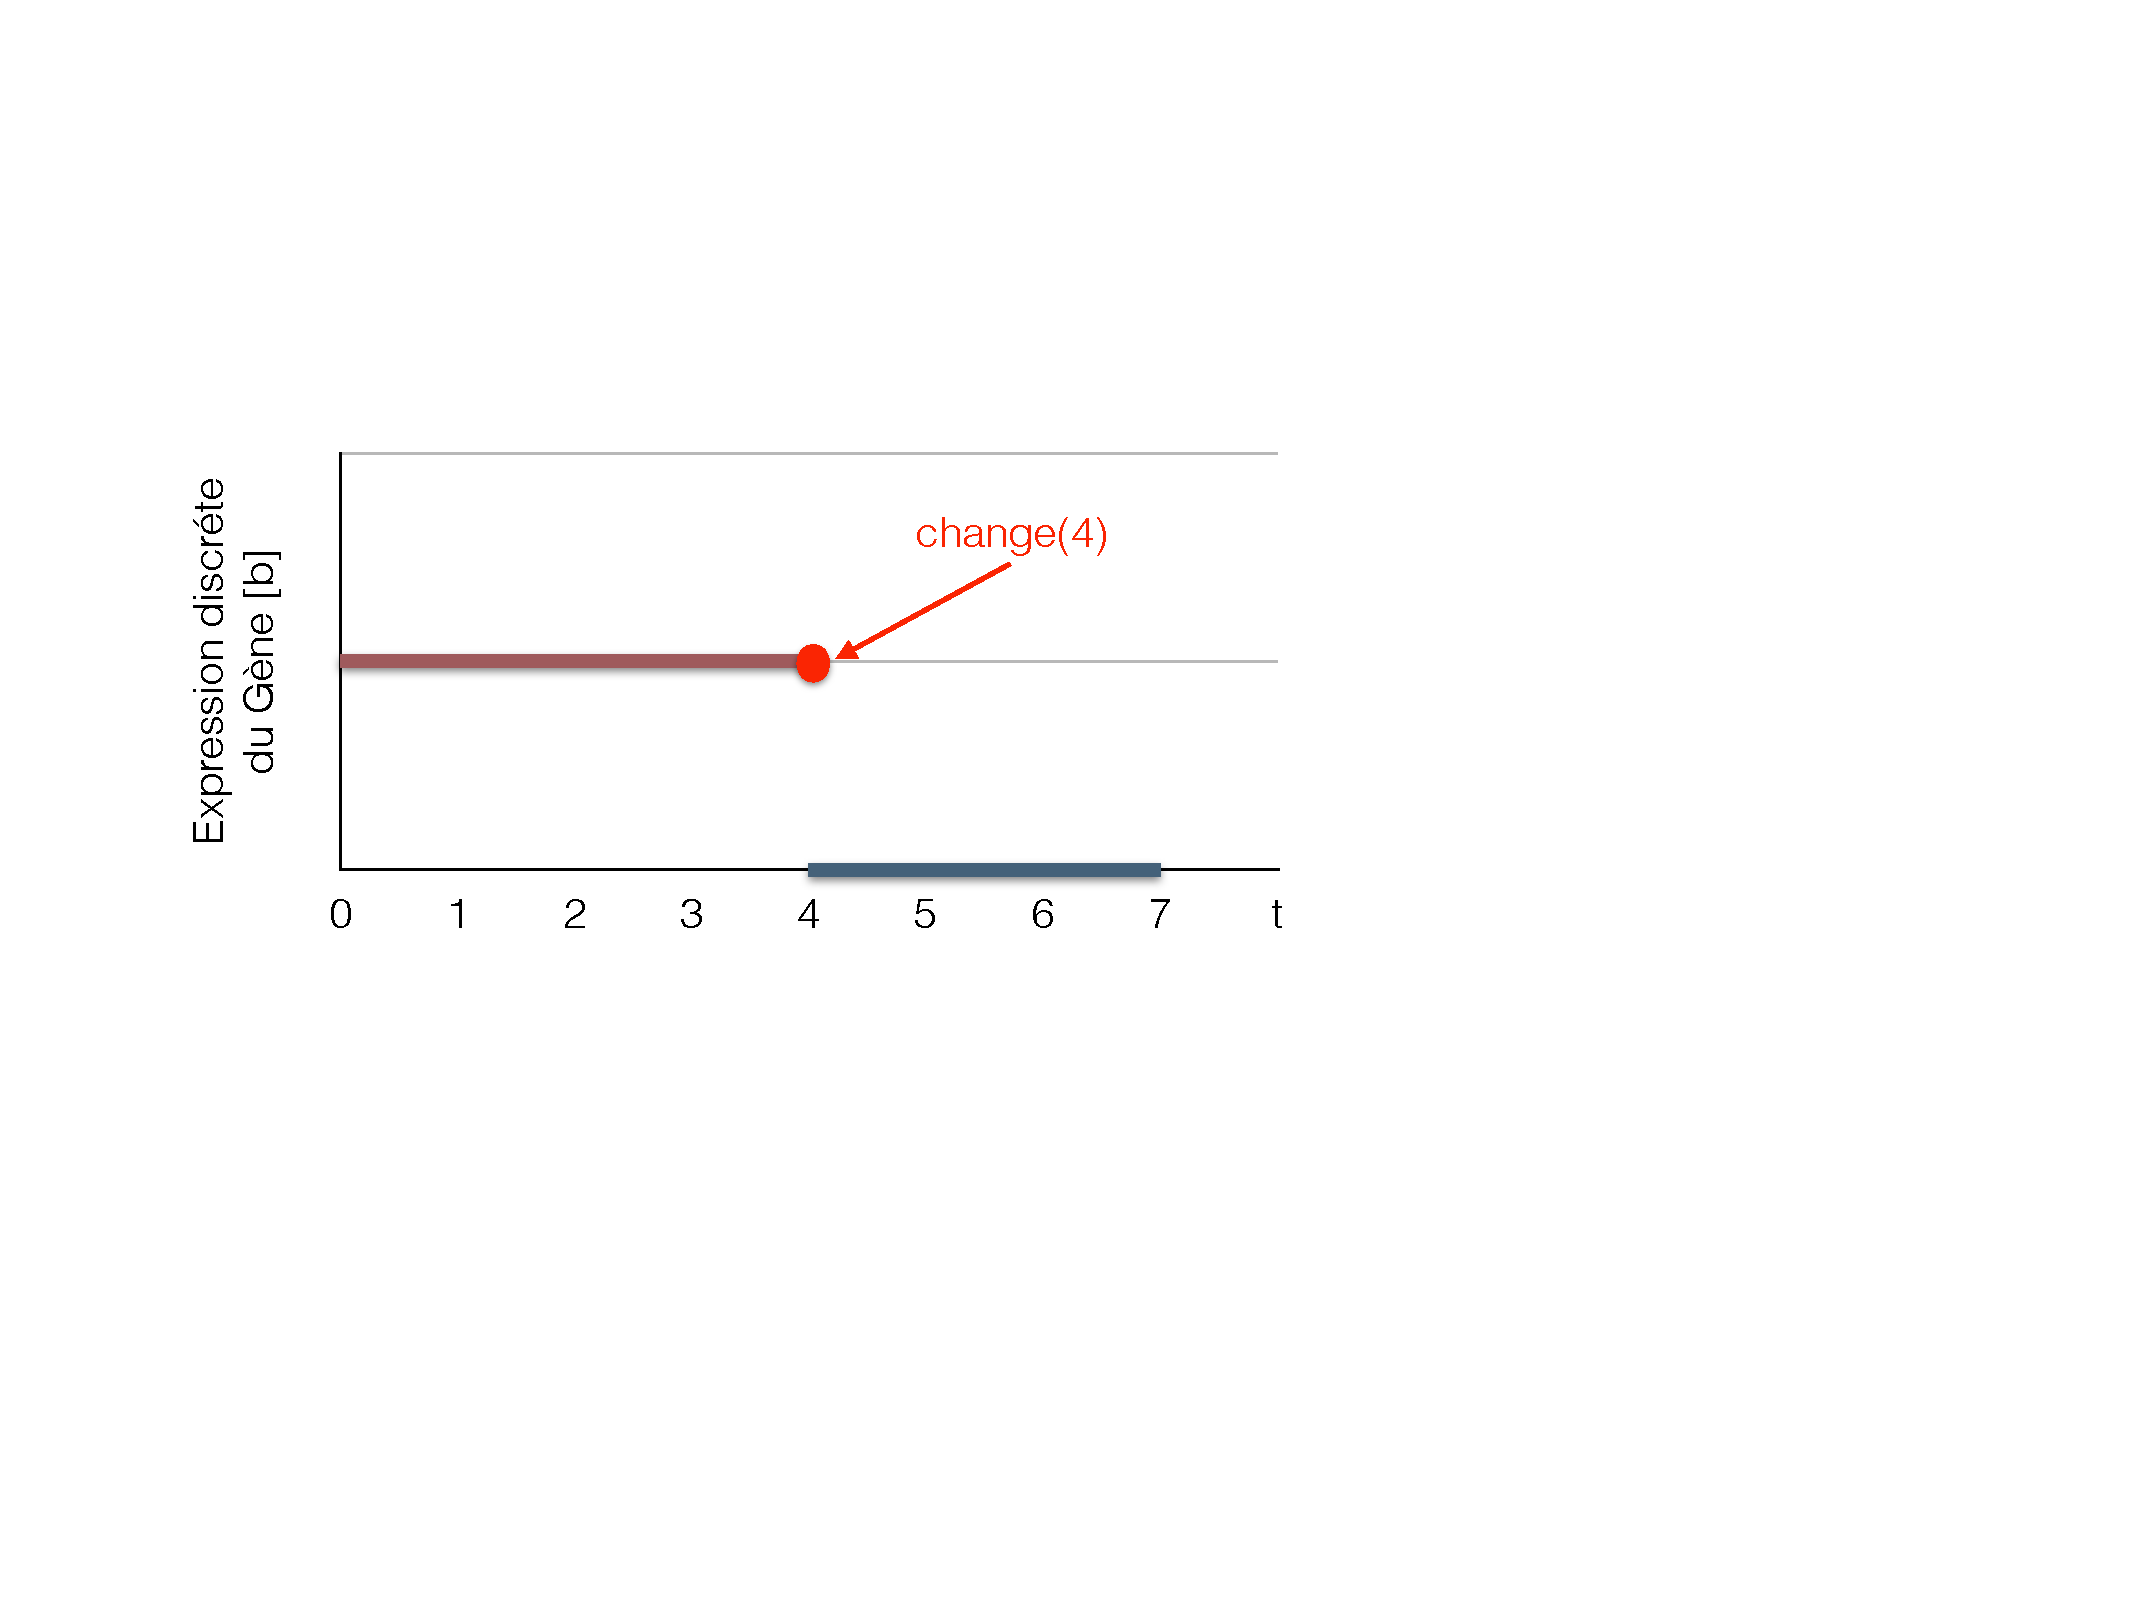
\includegraphics[width =0.31\linewidth]{images/courbes/gene-b-disc-change.pdf}
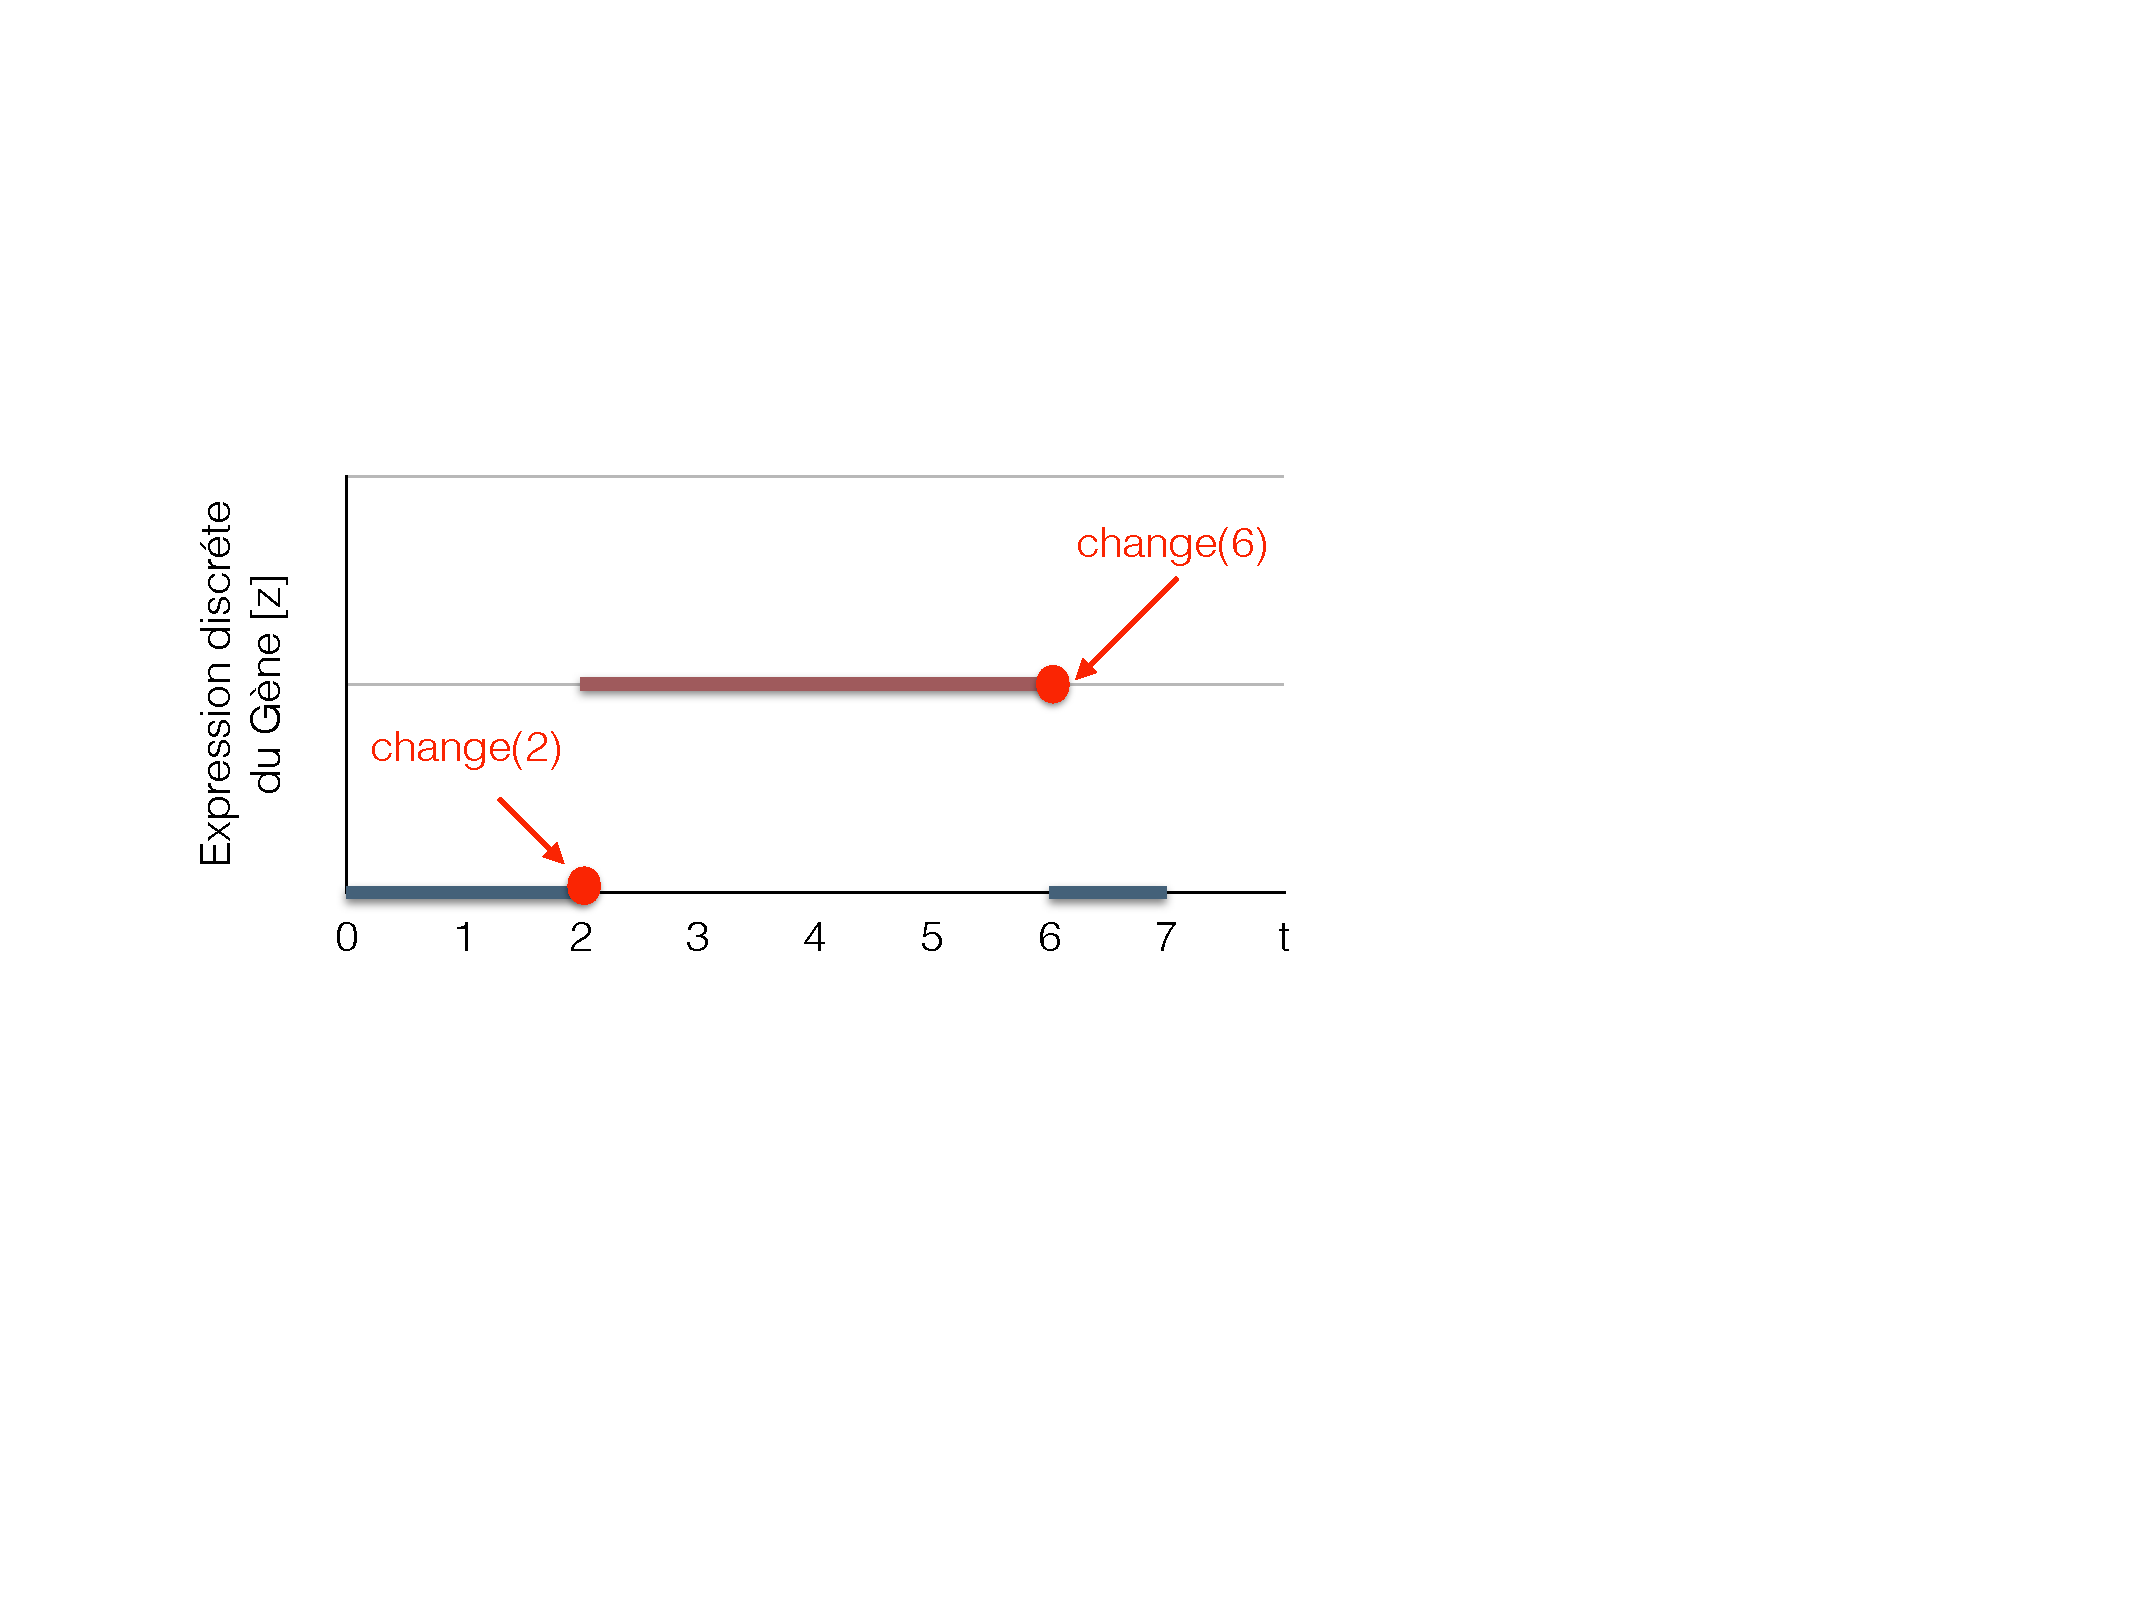
\includegraphics[width =0.31\linewidth]{images/courbes/gene-z-disc-change.pdf}
\caption{Examples of the discretization of continues time series data into bi-valued chronograms.
Abscisse represents time and ordinate the gene expression level.
The expression level is discretized according to a treshold fixed to the half of the gene expression value in this example.}
\end{figure}

\textcolor{red}{Summarry of the algorithm:}
\begin{itemize}
\item[-] Detection of changes
\item[-] Computation of the interactions possibly reponsible of those changes
PH:  \textit{action} : \textit{hitter(s)}, \textit{target} and \textit{delay}
\item[-] Filtering of the candidates actions
\item[-] Add actions to the model: completion/revision of the model
\end{itemize}

% Running example

Algorithm execution:

Let $i$ be the maximal number of hitters in an action of a PH: {\textit the indegree}.

The first change occurs at $t_1$ = $t_{min}$ = 2,
wich we will denote as \texttt{change(2)}.
It has been caused by an action $h = \PHfrappedelay{A}{D}{z_0}{z_1}$
where $ A \in \PHl^{\diamond}, | A| \leq i, i=2$ and $D$ is the delay wich is equal to 2 here since
$D_{t_i}=t_i - t_{i-1}$, such that $\exists$ \texttt{change($t_i$)} and \texttt{change($t_{i-1}$)},
$D_{t_1}= t_1 - t_0 = 2 - 0 = 2$.

Let $R=\{ b \rightarrow z, a \rightarrow z, a \rightarrow a \}$
be the set of regulation influences amoung the components of the system.
%
In the first change $t_1$ = 2 that we will denotes as $change(2)$,
its \texttt{z} whose value changes from $z_0$ to $z_1$, thus the action that has realized this change is of the form $h = \PHfrappedelay{A}{2}{z_0}{z_1}$. According to $R$ the genes which influence \texttt{z} are $G_{R_z} = \{\texttt{a, b}\}$. It means that $A= \{ a_{\textcolor{red}{?}}, b_{\textcolor{red}{?}} \} $ or $A= \{ a_{\textcolor{red}{?}} \} $ or $A= \{ b_{\textcolor{red}{?}} \} $
%
The expression level of the genes of $G{R_z}$ between $t_i$ and $t_{i-1}$ is as follows:
\begin{itemize}
\item[-] $a \in  G{R_z}$: $[a]_t=0$ $\forall t \in [0,2] $
\item[-] $b \in  G{R_z}$: $[b]_t=1$ $\forall t \in [0,2] $
\end{itemize}
%
Thus $A= \{ a_0, b_1 \} $ or $A= \{ a_0\} $ or $A= \{ b_1 \} $ and the set of candidate actions is:
$H_{change(2)} = \{ h_1=\PHfrappedelay{a_0}{2}{z_0}{z_1}
, h_2=\PHfrappedelay{b_1}{2}{z_0}{z_1}
, h_3=\PHfrappedelay{a_0 \wedge b_1 }{2}{z_0}{z_1} \}$.

The second change occurs at $t_2$ = 3 and we will denotes it as $change(3)$.
Here its \texttt{a} whose value changes from $a_0$ to $a_1$, thus the action that has realized this change is of the form
$h = \PHfrappedelay{A}{\textcolor{red}{D}}{a_0}{a_1}$ 
where $ A \in \PHl^{\diamond}, | A| \leq 2$ and $D$ is the delay that is equal to 1 here: 
$D_{t_2}= t_2 - t_1 = 3 - 2= 1$
According to $R$ the genes which influence \texttt{a} are $G_{R_a} = \{\texttt{a}\}$.
It means that $A= \{ a_{\textcolor{red}{?}}\}$ and the expression level of \texttt{a} between $t_1$ and $t_{2}$ is $a_0$.
Thus  $A= \{ a_0\} $ and there is only one candidate action that is a self action:
$H_{change(3)} = \{ h=\PHfrappedelay{a_0}{1}{a_0}{a_1}  \}$.

The third change occurs at $t_3$ = 4 and we will denotes it as $change(4)$.
Here its \texttt{b} whose value changes from $b_1$ to $b_0$, thus the action that has realized this change is of the form 
$h = \PHfrappedelay{A}{D}{b_1}{b_0}$ where $ A \in \PHl^{\diamond}, | A| \leq 2$ and $D$ is the delay that is equal to 1 here:
$D_{t_3}= t_3 - t_2 = 4 - 3 = 1$.
According to $R$ there is no genes that can influence \texttt{b}, thus no action can realize this change.

The fourth change occurs at $t_4$ = 5 and we will denotes it as $change(5)$.
Here its \texttt{a} whose value changes from $a_1$ to $a_0$, thus the action that has realized this change is of the form$h = \PHfrappedelay{A}{D}{a_1}{a_0}$ \\
where $ A \in \PHl^{\diamond}, | A| \leq 2$ and $D$ is the delay that is equal to 1 here:
$D_{t_4}= t_4 - t_3 = 5 - 4= 1$.
According to $R$ the genes which influence \texttt{a} are $G_{R_a} = \{\texttt{a}\}$.
Again $A= \{ a_{\textcolor{red}{?}}\}$ and since the expression level of \texttt{a} between $t_3$ and $t_{4}$ is $a_1$,
we have $A= \{ a_1\} $ and there is only one candidate action that is a self action:
$H_{change(5)} = \{ h=\PHfrappedelay{a_1}{1}{a_1}{a_0} \}$.

The fifth change occurs at $t_5$ = 6 and we will denotes it as $change(6)$.
Here its \texttt{z} whose value changes from $z_1$ to $z_0$, thus the action that has realized this change is of the form 
$h = \PHfrappedelay{A}{D}{z_1}{z_0}$ \\
where $ A \in \PHl^{\diamond}, |A| \leq 2$ and $D$ is equal to 1 here:
$D_{t_5}= t_5 - t_4 = 6 - 5= 1$ \\
According to $R$ the genes which influence \texttt{z} are $G_{R_z} = \{\texttt{a, b}\}$.
It means that $A= \{ a_{\textcolor{red}{?}}, b_{\textcolor{red}{?}} \} $ or $A= \{ a_{\textcolor{red}{?}} \} $ or $A= \{ b_{\textcolor{red}{?}} \} $
The expression level of \texttt{a} and \texttt{a} between $t_4$ and $t_{5}$ is respectively $a_0$ and $b_0$.
Thus $A= \{ a_0, b_1 \} $ or $A= \{ a_0\} $ or $A= \{ b_0 \} $ \\
The candidates action are: mon slip
$H_{change(6)} = \{ h_1=\PHfrappedelay{a_0}{1}{z_1}{z_0}$
, $  h_2=\PHfrappedelay{b_0}{1}{z_1}{z_0}$
, $  h_3=\PHfrappedelay{a_0 \wedge b_0 }{1}{z_1}{z_0} \}$.

After proccessing all chronograms, the candidates action are: \\
$H_{change(2)} = \{ h_1=\PHfrappedelay{a_0}{2}{z_0}{z_1}$, $  h_2=\PHfrappedelay{b_1}{2}{z_0}{z_1}$ \\
, \hspace{0.75cm}$  h_3=\PHfrappedelay{a_0 \wedge b_1 }{2}{z_0}{z_1} \}$.\\
$H_{change(3)} = \{ h=\PHfrappedelay{a_0}{1}{a_0}{a_1}  \}$. \\

$H_{change(5)} = \{ h=\PHfrappedelay{a_1}{1}{a_1}{a_0}  \}$. \\

$H_{change(6)} = \{ h_1=\PHfrappedelay{a_0}{1}{z_1}{z_0}$ , $  h_2=\PHfrappedelay{b_0}{1}{z_1}{z_0}$ \\
, \hspace{0.75cm} $  h_3=\PHfrappedelay{a_0 \wedge b_0 }{1}{z_1}{z_0} \}$. \\

At this stage of the process, all canditates actions are consistent with all observations and given regulation influences.
Until now the method used ensured completeness: here we have the complete set of consistent action that can explain the observations.
But in practice those set of action can be further refine using background knowledge.
The following filtering operation can help to reduce the complexity of the model learned/revised.

$1^{st}$ filter: \\

If we want to minimize the number of actions added to the input PH we can consider that the action of this PH are more trustable than the generated one. Thus generated actions that only explain changes that can already be explain by given action can be discarded: $\forall t \in T$ such that $\exists$  \texttt{change(t)}, we have:
\begin{itemize}
\item[-] \texttt{$H_c$}: the set of candidates action generated to explain $change(t)$
\item[-] \texttt{$H_{ini}$:} the set of actions of $PH_{ini}$ that can realize the change at $t$
\item[-] \texttt{$H_{final}$:} the set of actions to keep as to explain the change at $t$
\end{itemize}
We have either:
\begin{itemize}
\item[•] If $H_c \cap H_{ini} \neq \emptyset $ then $H_{final}= H_c \cap H_{ini}$ 
\item[•] If $H_c \cap H_{ini} = \emptyset $ then $H_{final}=H_c$
\end{itemize}
In practice, the change that already can be explained by the input PH can be detected before computing the candidates actions, allowing us to discard them without generating them.

$2^{nd}$ filter: \\

If knowledge about strict influences is given it can be used to discarded actions that are conflicting with those influences.
For example, if we know that a gene $a$ influences a gene $b$ and that $a$ can only inhibit $b$, then the actions using $a$ as hitter to increase the value of $b$ are inconsistent and can be discarded.
$\forall h \in H$ such $h=\PHfrappedelay{A}{D}{b_n}{b_m}$, with $ A \in \PHl^{\diamond}, | A| \leq i$ ($i$: indegree of the algorithm) we have :

\begin{itemize}
\item[•] If $n < m$, if $\exists G_k \in \PHl_G $ such that $G_k \xrightarrow{(-)} b$ (and $\nexists G_k \xrightarrow{(+)} b$ ) and $k \neq 0$ then $h$ can be discarded.
\item[•] If $n > m$, if $\exists G_k \in \PHl_G $ such that $G_k \xrightarrow{(+)} b$ (and $\nexists G_k \xrightarrow{(-)} b$ ) and $k \neq 0$ then $h$ can be discarded.
\end{itemize} 

$3^rd$ filter:\\

When the time information of observation is not perfect, the same regulation interaction may append with different delay.
One simple solution to deal with such input can be to simply agregate action that differ only by their delay.
We can merge each action with the same hitters, $S_1,P_1,\ldots, S_n,P_n$ and the same target, $G, P, P'$, into one action where the delay is the average.
$\forall h_1, h_2,..., h_k \in H$ such that $h_1=\PHfrappedelay{A}{D_1}{a_n}{a_m}$, $h_2=\PHfrappedelay{A}{D_2}{a_n}{a_m}$, ..., $h_k=\PHfrappedelay{A}{D_k}{a_n}{a_m}$ with $ A \in \PHl^{\diamond}$, $a_n, a_m \in \PHl_a$ et $D_1 \neq D_2 \neq ... \neq D_k$ then : \\
\texttt{fusion} all actions $h_1, h_2,..., h_k$ into one action $h$ $$h=\PHfrappedelay{A}{D_{average}}{a_n}{a_m}$$ such that: 
$$D_{average} = \frac{\sum_{i=1}^k D_{i}}{k} $$

 % % Evaluation de la méthode de la completion/revision des PH
\section{Evaluation}
\label{sec:evaluation}
\subsection{Application: Circadian clock}

Figure \ref{fig:circadian_clock} shows the circadian clock model of \cite{comet2012simplified}.
The right part shows a chronogram of the gene evolution of the circadian clock.
The abscisse axe represents time steps in hours and ordinate represents the gene value.
In this example we observe the evolution of genes $G$ and $PC$ during the night ($L$ is fixed to 0).
Here we can see the 7 (resp. 5) hours of delay shift of $PC$ (resp. $G$) from $1$ to $0$ and vice versa.
Indeed, $PC$ and $G$ respectively change their state $7$ hours and $5$ hours after a change occurs in the system.

\begin{figure}[tb]
\begin{center}
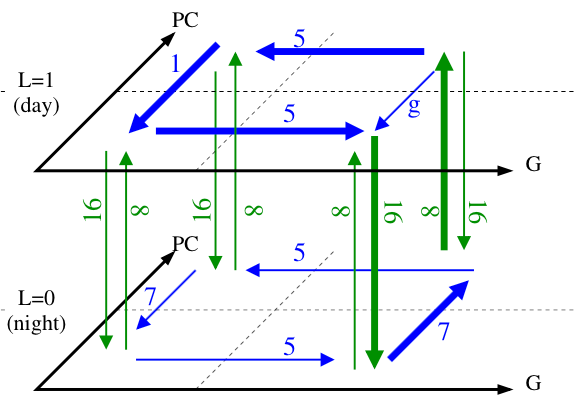
\includegraphics[width=0.4\linewidth]{images/circadianClock-summer.png}
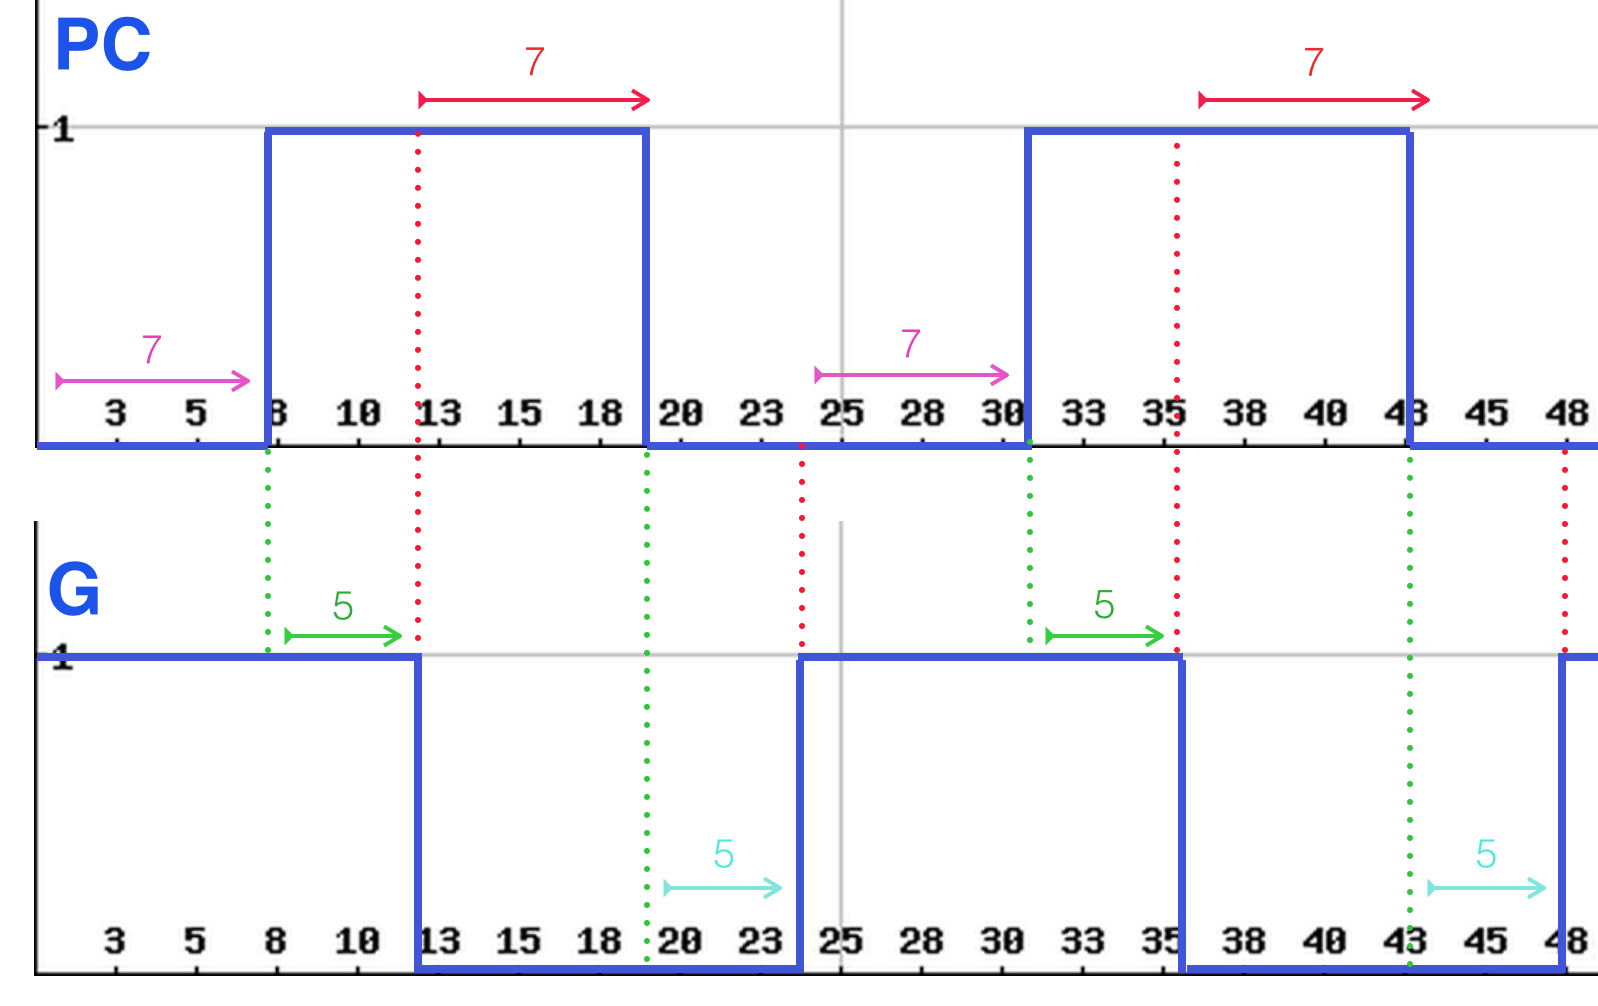
\includegraphics[width=0.4\linewidth]{images/circadianClock-Courb.png}
\end{center}
\caption{The first figure is taken from \cite{comet2010formal}, it presents the qualitative model of the mammalian circadian cycle during the summer. The second one is a chronogram corresponding to the discretization of the observed data set of a circadian clock components during the night (L=0).}
\label{fig:circadian_clock}
\end{figure}

The left part of \pref{fig:PH_circadian} shows the circadian clock represented as a Process Hitting with timed plural actions.
Here, the light $L$, the gene $PC$ and $G$ are represented by sorts with two processes.
The light clock is represented by an autonomous temporized sort: there are only auto-actions.
Actions are represented by edges as follows: when a node have incoming edge its the target of an action and the hitters of this action are the nodes where those edges are coming.
Each action is labelled by its delay.
Right part of the figure shows the representation of the circadian clock with the ASP formulation we presented in section \ref{sec:ph-asp}.



\subsection{Experiments}

In this section, we evaluate our approach on learning the circadian clock actions.
All experiments are run with a ASP implementation of Algorithm \ref{alg:PHC_ap} on a processor Intel Xeon (X5650, 2.67GHz) with 12GB of RAM.

	\begin{figure}[htb!]
	\vspace{1.5cm}
	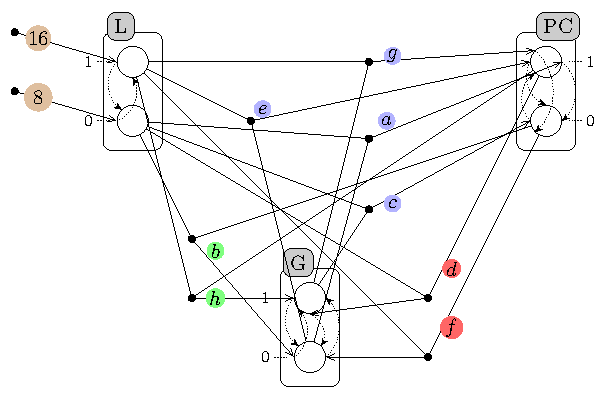
\includegraphics[width=0.6\linewidth]{images/circadianPH.pdf}
	%
	\hspace{0.1cm}
	%
	\begin{minipage}{0.32\linewidth}
	\vspace{-5cm}
		\textbf{Nodes:} \\
	\texttt{{\ssmall process("L",0..1).} }\\
	\texttt{{\ssmall process("PC",0..1).}}\\
	\texttt{{\ssmall process("G",0..1).} }\\
	\texttt{{\ssmall temporised("L").} }\\

	\textbf{Actions:} \\
	\texttt{{\ssmall action("L",0, "L",0,1,  8).}} ~\\
	\texttt{{\ssmall action("L",1, "L",1,0,  16).}} ~\\
	\texttt{{\ssmall action("L",0, "G",0, "PC",1,0,  a).}} ~\\
	\texttt{{\ssmall action("L",0, "PC",0, "G",0,1, b).}} ~\\
	\texttt{{\ssmall action("L",0, "G",1, "PC",0,1, c).}} ~\\
	\texttt{{\ssmall action("L",0, "PC",1, "G",1,0, d).}} \\
	\texttt{{\ssmall action("L",1, "G",0, "PC",1,0,  e).}} ~\\
	\texttt{{\ssmall action("L",1, "PC",0, "G",0,1, f).}} ~\\
	\texttt{{\ssmall action("L",1, "G",1, "PC",1,0, g).}} ~\\
	\texttt{{\ssmall action("L",1, "PC",1, "G",1,0, h).}} 

	\end{minipage}
	\caption{Representation of circadian clock in Process Hitting (left) and the equivalent ASP representation (right). The value $"a", "b", ..., "h"$ represent the delays in actions. }
		\label{fig:PH_circadian}

	\end{figure}
%

When the ASP representation of a chronogram like the one of Figure \ref{fig:circadian_clock} is given as input to Algorithm \ref{alg:PHC_ap} it will generate all the timed actions that can induce the observed changes.
The delay of the action is simply determined from the time delay between two changes.

\begin{figure}[htb!]
\begin{center}
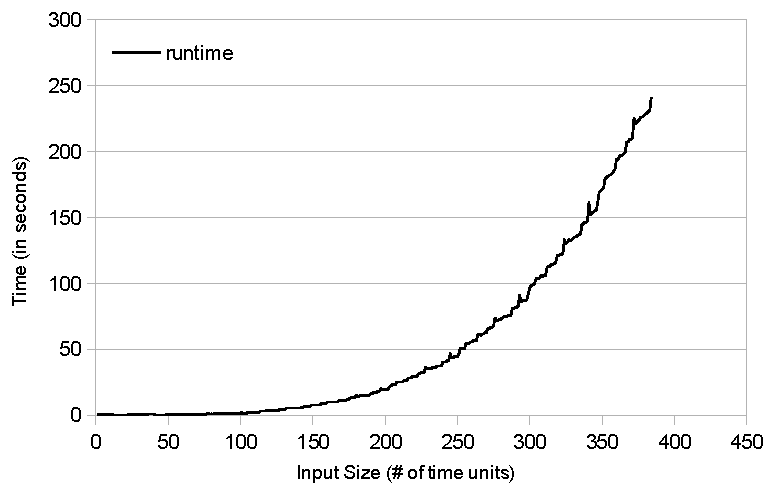
\includegraphics[width=0.5\linewidth]{images/circadian_run_time}
\end{center}
\caption{Run time of the application of Algorithm \ref{alg:PHC_ap} on circadian clock chronograms varying the number of time steps.}
\label{fig:run_time}
\end{figure}

Figure \ref{fig:run_time} shows the evolution of run time of our ASP implementation of Algorithm \ref{alg:PHC_ap} on the inference of the circadian clock actions regarding the quantity of input data.
In this experiment, we analyse the scalability of our approach by varying the number of time units of the input, i.e. the size of the chronogram.
Here we can see that the time needed to analyse the input data grows exponentially.
The experiments stop at 384 because the memory required by the ASP solver reached the 12GB of RAM we have.
It is currently quite difficult to obtain real data from biological system with chronogram exceeding 100 points.
In work like \cite{Fippo14} the considered chronograms are only composed of about 10 points.
Regarding the circadian clock, a chronogram of 100 data points is about 4 days of data, that is not much information, especially in cases where we want to analyze the effect of perturbations (for example, understand the recoverability phase in case of jet-lag). 
% TODO Morgan: Plus de blabla

  %\input{parts/circadianClock}
  \section{Conclusion and perspectives}
\label{sec:conclusion}

In this paper, we proposed an approach to automatically infer timed models of Process Hitting from time series data (expressed as chronograms). To do so, we implemented our algorithm in ASP. We illustrated the applicability and limits of the method through various benchmarks. This opens the way to promising applications in the connection between biologists and computer scientists. Further works will now consist in discussing the kind of information one can get on timed Process Hitting by analyzing the associated untimed model. We also plan to improve our implementation to make it robust against noisy data.  

%Nous avons montré dans cette thèse de Master une nouvelle analyse dynamique développée. Cette analyse est applicable à une classe de modèles dits PH et vise à déterminer des propriétés des réseaux modélisés. 

%La première propriété est la recherche des états stables du réseau qu'on appelle les points fixes. Ces points représentent les états du réseau pendant lesquels, le modèle ne peut plus évoluer. Il est intéressant à les connaitre car ils bloquent l'évolution des systèmes biologiques. Nous avons développé deux méthodes, sachant que la deuxième est plus optimale, qui retournent l'ensemble de tous les points fixes du réseau. Ce point fixe n'est qu'un état du réseau traduit en ASP par un niveau pour chaque composant, autrement un processus pour chaque sorte. \\
%La deuxième propriété est une propriété qui se base sur la dynamique du réseau: l'atteignabilité. Un réseau biologique évolue dans plusieurs sens qui peuvent aboutir ou pas à des états-objectifs. Notre nouvelle approche retourne les chemins exactes aboutissant à atteindre un niveau cible d'un composant du système. Ce chemin se traduit par un ensemble de changements successives des niveaux. En PH cela se traduit par de changements successifs de processus et c'est ce que nos méthodes retournent comme résultat. Il s'avére que la méthode itérative en ASP est plus optimale que celle en ASP normal. En effet il n'est pas nécessaire de prévoir le nombre de changements pour la méthode itérative et elle retourne le résultat plus rapidement (quelques seconde pour des réseau moyennement grand).

%Une comparaison a été faite par rapport à l'existant, \textsc{PINT} et la méthode de Rocca et al. Les résultats montrent que, par rapport à \textsc{PINT}, la méthode de recherche des points fixes est efficace, mais que pour l'accessibilité, elle l'est moins que prévu. Cependant aussi notre méthode retourne de plus le chemin d'atteignabilité. Elle offre la possibilité de poser des questions plus générales par rapport à \textsc{PINT} portant sur plusieurs sortes de plus. \\
%Sachant que la présentation d'un réseau biologique en PH est simplifie le traitement et la traduction des modèles, il s'avère que notre méthode qui se base sur ce formalisme est plus efficace que d'autres méthodes développées en ASP aussi mais pour des réseau de graphes de transitions. Le cas de la méthode de Rocca qui est gourmande en temps par rapport à la notre, résultat retourné en des minutes contre un résultat affiché en quelques secondes.\\

%Nous pensons que cette approche peut également être utilisée et adaptée avec d'autres modèles tels que le modèle de Thomas, les réseaux de Petri et les modèles synchrones. Cela nécessite une traduction propre au modèle étudié ainsi qu'un traitement approprié.\\
%Parmi nos perspectives qui font partie de mon sujet de thèse, c'est d'essayer d'améliorer cette méthode en éliminant les cycles de la méthode itérative. Cela évite de tourner indéfiniment dans des boucles sans avoir un résultat affiché.\\ 

%Ensuite, nous souhaitons étendre le programme pour chercher les attracteurs. Un attracteur est un ensemble d'états à partir desquels il n'est plus possible de sortir, et donc tel que le réseau tourne indéfiniment dans ces états. Le point fixe est un cas spécial des attracteur, en effet c'est un attracteur de dimension une. Par contre, la caractérisation des attracteurs  de la dynamique,de dimension $n$, requiert une analyse des dynamiques possibles bien plus poussée que pour les points fixes.\\
%Nous visons aussi à implémenter une recherche dynamique dans le sens inverse de l'atteignabilité et poser la question: "\textit{Quels sont les états initiaux qui nous permettent d'atteindre nos objectifs?}".  La réponse à cette question est l'ensemble des états à partir des quels il existe des chemins qui activent le ou les objectif(s). C'est vrai que la méthode de Rocca et al. résolve cette problématique mais nous estimons à avoir une approche plus efficace en terme de temps et qui utilise le réseau en process hitting en non pas les graphes de transitions.

%Tous ces problématiques constituent une perspective intéressante dans le cadre du développement de techniques d'analyse statique et dynamiques des propriétés du Process Hitting.\\

  \bibliographystyle{plain}
  \bibliography{biblio}

%\section*{Appendix: Springer-Author Discount}

\end{document}
